% Options for packages loaded elsewhere
\PassOptionsToPackage{unicode}{hyperref}
\PassOptionsToPackage{hyphens}{url}
%
\documentclass[
]{article}
\usepackage{lmodern}
\usepackage{amssymb,amsmath}
\usepackage{ifxetex,ifluatex}
\ifnum 0\ifxetex 1\fi\ifluatex 1\fi=0 % if pdftex
  \usepackage[T1]{fontenc}
  \usepackage[utf8]{inputenc}
  \usepackage{textcomp} % provide euro and other symbols
\else % if luatex or xetex
  \usepackage{unicode-math}
  \defaultfontfeatures{Scale=MatchLowercase}
  \defaultfontfeatures[\rmfamily]{Ligatures=TeX,Scale=1}
\fi
% Use upquote if available, for straight quotes in verbatim environments
\IfFileExists{upquote.sty}{\usepackage{upquote}}{}
\IfFileExists{microtype.sty}{% use microtype if available
  \usepackage[]{microtype}
  \UseMicrotypeSet[protrusion]{basicmath} % disable protrusion for tt fonts
}{}
\usepackage{xcolor}
\IfFileExists{xurl.sty}{\usepackage{xurl}}{} % add URL line breaks if available
\IfFileExists{bookmark.sty}{\usepackage{bookmark}}{\usepackage{hyperref}}
\hypersetup{
  pdftitle={Bootstrapping statistics of the maximum likelihood estimator of components in a series systems from masked failure data},
  pdfauthor={Alex Towell},
  hidelinks,
  pdfcreator={LaTeX via pandoc}}
\urlstyle{same} % disable monospaced font for URLs
\usepackage[margin=1in]{geometry}
\usepackage{color}
\usepackage{fancyvrb}
\newcommand{\VerbBar}{|}
\newcommand{\VERB}{\Verb[commandchars=\\\{\}]}
\DefineVerbatimEnvironment{Highlighting}{Verbatim}{commandchars=\\\{\}}
% Add ',fontsize=\small' for more characters per line
\usepackage{framed}
\definecolor{shadecolor}{RGB}{248,248,248}
\newenvironment{Shaded}{\begin{snugshade}}{\end{snugshade}}
\newcommand{\AlertTok}[1]{\textcolor[rgb]{0.94,0.16,0.16}{#1}}
\newcommand{\AnnotationTok}[1]{\textcolor[rgb]{0.56,0.35,0.01}{\textbf{\textit{#1}}}}
\newcommand{\AttributeTok}[1]{\textcolor[rgb]{0.77,0.63,0.00}{#1}}
\newcommand{\BaseNTok}[1]{\textcolor[rgb]{0.00,0.00,0.81}{#1}}
\newcommand{\BuiltInTok}[1]{#1}
\newcommand{\CharTok}[1]{\textcolor[rgb]{0.31,0.60,0.02}{#1}}
\newcommand{\CommentTok}[1]{\textcolor[rgb]{0.56,0.35,0.01}{\textit{#1}}}
\newcommand{\CommentVarTok}[1]{\textcolor[rgb]{0.56,0.35,0.01}{\textbf{\textit{#1}}}}
\newcommand{\ConstantTok}[1]{\textcolor[rgb]{0.00,0.00,0.00}{#1}}
\newcommand{\ControlFlowTok}[1]{\textcolor[rgb]{0.13,0.29,0.53}{\textbf{#1}}}
\newcommand{\DataTypeTok}[1]{\textcolor[rgb]{0.13,0.29,0.53}{#1}}
\newcommand{\DecValTok}[1]{\textcolor[rgb]{0.00,0.00,0.81}{#1}}
\newcommand{\DocumentationTok}[1]{\textcolor[rgb]{0.56,0.35,0.01}{\textbf{\textit{#1}}}}
\newcommand{\ErrorTok}[1]{\textcolor[rgb]{0.64,0.00,0.00}{\textbf{#1}}}
\newcommand{\ExtensionTok}[1]{#1}
\newcommand{\FloatTok}[1]{\textcolor[rgb]{0.00,0.00,0.81}{#1}}
\newcommand{\FunctionTok}[1]{\textcolor[rgb]{0.00,0.00,0.00}{#1}}
\newcommand{\ImportTok}[1]{#1}
\newcommand{\InformationTok}[1]{\textcolor[rgb]{0.56,0.35,0.01}{\textbf{\textit{#1}}}}
\newcommand{\KeywordTok}[1]{\textcolor[rgb]{0.13,0.29,0.53}{\textbf{#1}}}
\newcommand{\NormalTok}[1]{#1}
\newcommand{\OperatorTok}[1]{\textcolor[rgb]{0.81,0.36,0.00}{\textbf{#1}}}
\newcommand{\OtherTok}[1]{\textcolor[rgb]{0.56,0.35,0.01}{#1}}
\newcommand{\PreprocessorTok}[1]{\textcolor[rgb]{0.56,0.35,0.01}{\textit{#1}}}
\newcommand{\RegionMarkerTok}[1]{#1}
\newcommand{\SpecialCharTok}[1]{\textcolor[rgb]{0.00,0.00,0.00}{#1}}
\newcommand{\SpecialStringTok}[1]{\textcolor[rgb]{0.31,0.60,0.02}{#1}}
\newcommand{\StringTok}[1]{\textcolor[rgb]{0.31,0.60,0.02}{#1}}
\newcommand{\VariableTok}[1]{\textcolor[rgb]{0.00,0.00,0.00}{#1}}
\newcommand{\VerbatimStringTok}[1]{\textcolor[rgb]{0.31,0.60,0.02}{#1}}
\newcommand{\WarningTok}[1]{\textcolor[rgb]{0.56,0.35,0.01}{\textbf{\textit{#1}}}}
\usepackage{longtable,booktabs}
% Correct order of tables after \paragraph or \subparagraph
\usepackage{etoolbox}
\makeatletter
\patchcmd\longtable{\par}{\if@noskipsec\mbox{}\fi\par}{}{}
\makeatother
% Allow footnotes in longtable head/foot
\IfFileExists{footnotehyper.sty}{\usepackage{footnotehyper}}{\usepackage{footnote}}
\makesavenoteenv{longtable}
\usepackage{graphicx}
\makeatletter
\def\maxwidth{\ifdim\Gin@nat@width>\linewidth\linewidth\else\Gin@nat@width\fi}
\def\maxheight{\ifdim\Gin@nat@height>\textheight\textheight\else\Gin@nat@height\fi}
\makeatother
% Scale images if necessary, so that they will not overflow the page
% margins by default, and it is still possible to overwrite the defaults
% using explicit options in \includegraphics[width, height, ...]{}
\setkeys{Gin}{width=\maxwidth,height=\maxheight,keepaspectratio}
% Set default figure placement to htbp
\makeatletter
\def\fps@figure{htbp}
\makeatother
\setlength{\emergencystretch}{3em} % prevent overfull lines
\providecommand{\tightlist}{%
  \setlength{\itemsep}{0pt}\setlength{\parskip}{0pt}}
\setcounter{secnumdepth}{5}
\usepackage{graphicx}
\usepackage{amsthm}
\usepackage{amsmath}
\usepackage{natbib}
\usepackage{tikz}
\usepackage[]{natbib}
\bibliographystyle{apalike}
\newlength{\cslhangindent}
\setlength{\cslhangindent}{1.5em}
\newenvironment{cslreferences}%
  {}%
  {\par}

\title{Bootstrapping statistics of the maximum likelihood estimator of
components in a series systems from masked failure data}
\author{Alex Towell}
\date{}

\begin{document}
\maketitle
\begin{abstract}
We estimate the parameters of a series system with Weibull component
lifetimes from relatively small samples consisting of right-censored
system lifetimes and masked component cause of failure. Under a set of
conditions that permit us to ignore how the component cause of failures
are masked, we assess the bias and variance of the estimator. Then, we
assess the accuracy of the boostrapped variance and calibration of the
confidence intervals of the MLE under a variety of scenarios.
\end{abstract}

{
\setcounter{tocdepth}{2}
\tableofcontents
}
\newcommand{\T}{T}
\newtheorem{definition}{Definition}
\newtheorem{theorem}{Theorem}
\newtheorem{corollary}{Corollary}
\newtheorem{condition}{Condition}
\renewcommand{\v}[1]{\boldsymbol{#1}}
\numberwithin{equation}{section}

\hypertarget{introduction}{%
\section{Introduction}\label{introduction}}

Accurately estimating the reliability of individual components in
multi-component systems is an important problem in many engineering
domains. However, component lifetimes and failure causes are often not
directly observable. In a series system, only the system-level failure
time may be recorded along with limited information about which
component failed. Such \emph{masked} data poses challenges for
estimating component reliability.

In this paper, we develop a maximum likelihood approach to estimate
component reliability in series systems using right-censored lifetime
data and candidate sets that contain the failed component. The key
contributions are:

\begin{enumerate}
\def\labelenumi{\arabic{enumi}.}
\item
  Deriving a likelihood model that accounts for right-censoring and
  masked failure causes through candidate sets. This allows the
  available masked data to be used for estimation.
\item
  Validating the accuracy, precision, and robustness of the maximum
  likelihood estimator through an extensive simulation study under
  different sample sizes, masking probabilities, and censoring levels.
\item
  Demonstrating that bootstrapping provides well-calibrated confidence
  intervals for the MLEs even with small samples.
\end{enumerate}

Together, these contributions provide a statistically rigorous
methodology for learning about latent component properties from series
system data. The methods are shown to work well even when failure
information is significantly masked. This capability expands the range
of applications where component reliability can be quantified from
limited observations.

The remainder of this paper is organized as follows. First, we detail
the series system and masked data models. Next, we present the
likelihood construction and maximum likelihood theory. We then describe
the bootstrap approach for variance and confidence interval estimation.
Finally, we validate the methods through simulation studies under
various data scenarios and sample sizes.

\hypertarget{sec:statmod}{%
\section{Series System Model}\label{sec:statmod}}

Consider a system composed of \(m\) components arranged in a series
configuration. Each component and system has two possible states,
functioning or failed. We have \(n\) systems whose lifetimes are
independent and identically distributed (i.i.d.). The lifetime of the
\(i\)\textsuperscript{th} system denoted by the random variable
\(T_{i}\). The lifetime of the \(j\)\textsuperscript{th} component in
the \(i\)\textsuperscript{th} system is denoted by the random variable
\(T_{i j}\). We assume the component lifetimes in a single system are
statistically independent and non-identically distributed. Here,
lifetime is defined as the elapsed time from when the new, functioning
component (or system) is put into operation until it fails for the first
time. A series system fails when any component fails, thus the lifetime
of the \(i\)\textsuperscript{th} system is given by the component with
the shortest lifetime, \[
    T_i = \min\bigr\{T_{i 1},T_{i 2}, \ldots, T_{i m} \bigr\}.
\]

There are three particularly important distribution functions in
survival analysis: the survival function, the probability density
function, and the hazard function. The survival function,
\(R_{T_i}(t)\), is the probability that the \(i\)\textsuperscript{th}
system has a lifespan larger than a duration \(t\), \begin{equation}
R_{T_i}(t) = \Pr\{T_i > t\}\\
\end{equation} The probability density function (pdf) of \(T_i\) is
denoted by \(f_{T_i}(t)\) and may be defined as \[
    f_{T_i}(t) = -\frac{d}{dt} R_{T_i}(t).
\] Next, we introduce the hazard function. The probability that a
failure occurs between \(t\) and \(\Delta t\) given that no failure
occurs before time \(t\) is given by \[
\Pr\{T_i \leq t+\Delta t|T_i > t\} = \frac{\Pr\{t < T_i < t+\Delta t\}}{\Pr\{T_i > t\}}.
\] The failure rate is given by the dividing this equation by the length
of the time interval, \(\Delta t\): \[
\frac{\Pr\{t < T < t+\Delta t\}}{\Delta t} \frac{1}{\Pr\{T > t\}} =
    \frac{R_T(t) - R(t+\Delta t)}{R_T(t)}.
\] The hazard function \(h_{T_i}(t)\) for \(T_i\) is the instantaneous
failure rate at time \(t\), which is given by \begin{equation}
\label{eq:failure_rate}
\begin{split}
h_{T_i}(t) &= \lim_{\Delta t \to 0} \frac{\Pr\{t < T_i < t+\Delta t\}}{\Delta t} \frac{1}{\Pr\{T_i > t\}}\\
       &= \frac{f_{T_i}(t)}{R_{T_i}(t)}.
\end{split}
\end{equation} \textbackslash end\{definition\}

The lifetime of the \(j\)\textsuperscript{th} component is assumed to
follow a parametric distribution indexed by a parameter vector
\(\boldsymbol{\theta_j}\). The parameter vector of the overall system is
defined as \[
    \boldsymbol{\theta }= (\boldsymbol{\theta_1},\ldots,\boldsymbol{\theta_m}).
\]

When a random variable \(T\) is parameterized by a particular
\(\boldsymbol{\theta}\), we denote the reliability function by
\(R_T(t;\boldsymbol{\theta})\), and the same for other distribution
functions. If it is clear from the context which random variable a
distribution function is for, we drop the subscripts, e.g., \(R(t)\)
instead of \(R_T(t)\). As a special case, we denote the pdf of the
\(j\)\textsuperscript{th} component by \(f_j(t;\boldsymbol{\theta_j})\)
and its reliability function by \(R_j(t;\boldsymbol{\theta_j})\).

Two random variables \(X\) and \(Y\) have a joint pdf \(f_{X,Y}(x,y)\).
Given the joint pdf \(f(x,y)\), the marginal pdf of \(X\) is given by \[
f_X(x) = \int_{\mathcal{Y}} f_{X,Y}(x,y) dy,
\] where \(\mathcal{Y}\) is the support of \(Y\). (If \(Y\) is discrete,
replace the integration with a summation over \(\mathcal{Y}\).)

The conditional pdf of \(Y\) given \(X=x\), \(f_{Y|X}(y|x)\), is defined
as \[
f_{X|Y}(y|x) = \frac{f_{X,Y}(x,y)}{f_X(x)}.
\] We may generalize all of the above to more than two random variables,
e.g., the joint pdf of \(X_1,\ldots,X_m\) is denoted by
\(f(x_1,\ldots,x_m)\).

Next, we dive deeper into these concepts and provide mathematical
derivations for the reliability function, pdf, and hazard function of
the series system. We begin with the reliability function of the series
system, as given by the following theorem.

\begin{theorem}
\label{thm:sys_reliability_function}
The series system has a reliability function given by
\begin{equation}
\label{eq:sys_reliability_function}
  R(t;\boldsymbol{\theta}) = \prod_{j=1}^m R_j(t;\boldsymbol{\theta_j}).
\end{equation}
\end{theorem}
\begin{proof}
The reliability function is defined as
$$
  R(t;\boldsymbol{\theta}) = \Pr\{T_i > t\}
$$
which may be rewritten as
$$
  R(t;\boldsymbol{\theta}) = \Pr\{\min\{T_{i 1},\ldots,T_{i m}\} > t\}.
$$
For the minimum to be larger than $t$, every component must be larger than $t$,
$$
  R(t;\boldsymbol{\theta}) = \Pr\{T_{i 1} > t,\ldots,T_{i m} > t\}.
$$
Since the component lifetimes are independent, by the product rule the above may
be rewritten as
$$
  R(t;\boldsymbol{\theta}) = \Pr\{T_{i 1} > t\} \times \cdots \times \Pr\{T_{i m} > t\}.
$$
By definition, $R_j(t;\boldsymbol{\theta}) = \Pr\{T_{i j} > t\}$.
Performing this substitution obtains the result
$$
  R(t;\boldsymbol{\theta}) = \prod_{j=1}^m R_j(t;\boldsymbol{\theta_j}).
$$
\end{proof}

Theorem \ref{thm:sys_reliability_function} shows that the system's
overall reliability is the product of the reliabilities of its
individual components. This property is inherent to series systems and
will be used in the subsequent derivations.

Next, we turn our attention to the pdf of the system lifetime, described
in the following theorem.

\begin{theorem}
\label{thm:sys_pdf}
The series system has a pdf given by
\begin{equation}
\label{eq:sys_pdf}
f(t;\boldsymbol{\theta}) = \sum_{j=1}^m f_j(t;\boldsymbol{\theta_j})
    \prod_{\substack{k=1\\k\neq j}}^m R_k(t;\boldsymbol{\theta_j}).
\end{equation}
\end{theorem}
\begin{proof}
By definition, the pdf may be written as
$$
    f(t;\boldsymbol{\theta}) = -\frac{d}{dt} \prod_{j=1}^m R_j(t;\boldsymbol{\theta_j}).
$$
By the product rule, this may be rewritten as
\begin{align*}
  f(t;\boldsymbol{\theta})
    &= -\frac{d}{dt} R_1(t;\boldsymbol{\theta_1})\prod_{j=2}^m R_j(t;\boldsymbol{\theta_j}) -
      R_1(t;\boldsymbol{\theta_1}) \frac{d}{dt} \prod_{j=2}^m R_j(t;\boldsymbol{\theta_j})\\
    &= f_1(t;\boldsymbol{\theta}) \prod_{j=2}^m R_j(t;\boldsymbol{\theta_j}) -
      R_1(t;\boldsymbol{\theta_1}) \frac{d}{dt} \prod_{j=2}^m R_j(t;\boldsymbol{\theta_j}).
\end{align*}
Recursively applying the product rule $m-1$ times results in
$$
f(t;\boldsymbol{\theta}) = \sum_{j=1}^{m-1} f_j(t;\boldsymbol{\theta_j})
    \prod_{\substack{k=1\\k \neq j}}^m R_k(t;\boldsymbol{\theta_k}) -
    \prod_{j=1}^{m-1} R_j(t;\boldsymbol{\theta_j}) \frac{d}{dt} R_m(t;\boldsymbol{\theta_m}),
$$
which simplifies to
$$
f(t;\boldsymbol{\theta})= \sum_{j=1}^m f_j(t;\boldsymbol{\theta_j})
    \prod_{\substack{k=1\\k \neq j}}^m R_k(t;\boldsymbol{\theta_k}).
$$
\end{proof}

Theorem \ref{thm:sys_pdf} shows the pdf of the system lifetime as a
function of the pdfs and reliabilities of its components.

We continue with the hazard function of the system lifetime, defined in
the next theorem.

\begin{theorem}
\label{thm:sys_failure_rate}
The series system has a hazard function given by
\begin{equation}
\label{eq:sys_failure_rate}
  h(t;\boldsymbol{\theta}) = \sum_{j=1}^m h_j(t;\boldsymbol{\theta_j}).
\end{equation}
\end{theorem}
\begin{proof}
By Equation \eqref{eq:failure_rate}, the $i$\textsuperscript{th} series system lifetime has a hazard function defined as
$$
  h(t;\boldsymbol{\theta}) = \frac{f_{T_i}(t;\boldsymbol{\theta})}{R_{T_i}(t;\boldsymbol{\theta})}.
$$
Plugging in expressions for these functions results in
$$
  h(t;\boldsymbol{\theta}) = \frac{\sum_{j=1}^m f_j(t;\boldsymbol{\theta_j})
    \prod_{\substack{k=1\\k \neq j}}^m R_k(t;\boldsymbol{\theta_k})}
      {\prod_{j=1}^m R_j(t;\boldsymbol{\theta_j})},
$$
which can be simplified to
$$
h_{T_i}(t;\boldsymbol{\theta}) = \sum_{j=1}^m \frac{f_j(t;\boldsymbol{\theta_j})}{R_j(t;\boldsymbol{\theta_j})} = \sum_{j=1}^m h_j(t;\boldsymbol{\theta_j}).
$$
\end{proof}

Theorem \ref{thm:sys_failure_rate} reveals that the system's hazard
function is the sum of the hazard functions of its components.

By definition, the hazard function is the ratio of the pdf to the
reliability function, \[
h(t;\boldsymbol{\theta}) = \frac{f(t;\boldsymbol{\theta})}{R(t;\boldsymbol{\theta})},
\] and we can rearrange this to get \begin{equation}
\label{eq:sys_pdf_2}
\begin{split}
f(t;\boldsymbol{\theta}) &= h(t;\boldsymbol{\theta}) R(t;\boldsymbol{\theta})\\
              &= \biggl\{\sum_{j=1}^m h_j(t;\boldsymbol{\theta_j})\biggr\}
                 \biggl\{ \prod_{j=1}^m R_j(t;\boldsymbol{\theta_j}) \biggr\},
\end{split}
\end{equation} which we sometimes find to be a more convenient form than
Equation \eqref{eq:sys_pdf}.

In this section, we derived the mathematical forms for the system's
reliability function, pdf, and hazard function. Next, we build upon
these concepts to derive distributions related to the component cause of
failure.

\hypertarget{sec:comp_cause}{%
\subsection{Component Cause of Failure}\label{sec:comp_cause}}

Whenever a series system fails, precisely one of the components is the
cause. We model the component cause of the series system failure as a
random variable.

\begin{definition}
The component cause of failure of a series system is
denoted by the random variable $K_i$ whose support is given by $\{1,\ldots,m\}$.
For example, $K_i=j$ indicates that the component indexed by $j$ failed first, i.e.,
$$
    T_{i j} < T_{i j'}
$$
for every $j'$ in the support of $K_i$ except for $j$.
Since we have series systems, $K_i$ is unique.
\end{definition}

The system lifetime and the component cause of failure has a joint
distribution given by the following theorem.

\begin{theorem}
\label{thm:f_k_and_t}
The joint pdf of the component cause of failure $K_i$ and series system lifetime
$T_i$ is given by
\begin{equation}
\label{eq:f_k_and_t}
  f_{K_i,T_i}(j,t;\boldsymbol{\theta}) = h_j(t;\boldsymbol{\theta_j}) R_{T_i}(t;\boldsymbol{\theta}),
\end{equation}
where $h_j(t;\boldsymbol{\theta_j})$ is the hazard function of the $j$\textsuperscript{th}
component and $R_{T_i}(t;\boldsymbol{\theta})$ is the reliability function of the series
system.
\end{theorem}
\begin{proof}
Consider a series system with $3$ components.
By the assumption that component lifetimes are mutually independent,
the joint pdf of $T_{i 1},T_{i 2},T_{i 3}$ is given by
$$
    f(t_1,t_2,t_3;\boldsymbol{\theta}) = \prod_{j=1}^{3} f_j(t;\boldsymbol{\theta_j}).
$$
The first component is the cause of failure at time $t$ if $K_i = 1$ and
$T_i = t$, which may be rephrased as the likelihood that $T_{i 1} = t$,
$T_{i 2} > t$, and $T_{i 3} > t$. Thus,
\begin{align*}
f_{K_i,T_i}(j;\boldsymbol{\theta}) 
    &= \int_t^{\infty} \int_t^{\infty}
        f_1(t;\boldsymbol{\theta_1}) f_2(t_2;\boldsymbol{\theta_2}) f_3(t_3;\boldsymbol{\theta_3})
        dt_3 dt_2\\
     &= \int_t^{\infty} f_1(t;\boldsymbol{\theta_1}) f_2(t_2;\boldsymbol{\theta_2})
        R_3(t;\boldsymbol{\theta_3}) dt_2\\
     &= f_1(t;\boldsymbol{\theta_1}) R_2(t;\boldsymbol{\theta_2}) R_3(t_1;\boldsymbol{\theta_3}).
\end{align*}
Since $h_1(t;\boldsymbol{\theta_1}) = f_1(t;\boldsymbol{\theta_1}) / R_1(t;\boldsymbol{\theta_1})$,
$$
f_1(t;\boldsymbol{\theta_1}) = h_1(t;\boldsymbol{\theta_1}) R_1(t;\boldsymbol{\theta_1}).
$$
Making this substitution into the above expression for $f_{K_i,T_i}(j,t;\boldsymbol{\theta})$
yields
\begin{align*}
f_{K_i,T_i}(j,t;\boldsymbol{\theta})
    &= h_1(t;\boldsymbol{\theta_1}) \prod_{l=1}^m R_l(t;\boldsymbol{\theta_l})\\
    &= h_1(t;\boldsymbol{\theta_1}) R(t;\boldsymbol{\theta}).
\end{align*}
Generalizing from this completes the proof.
\end{proof}

\hypertarget{sec:like_model}{%
\section{Likelihood Model for Masked Data}\label{sec:like_model}}

The object of interest is the (unknown) parameter value
\(\boldsymbol{\theta}\). To estimate this \(\boldsymbol{\theta}\), we
need \emph{data}. In our case, we call it \emph{masked data} because we
do not necessarily observe the event of interest, say a system failure,
directly. We consider two types of masking: masking the system failure
lifetime and masking the component cause of failure.

We generally encounter three types of system failure lifetime masking:

\begin{enumerate}
\def\labelenumi{\arabic{enumi}.}
\tightlist
\item
  A system failure is observed at a particular point in time.
\item
  A system failure is observed to occur within a particular interval of
  time.
\item
  A system failure is not observed, but we know that the system survived
  at least until a particular point in time. This is known as
  \emph{right-censoring} and can occur if, for instance, an experiment
  is terminated while the system is still functioning.
\end{enumerate}

We generally encounter two types of component cause of failure masking:

\begin{enumerate}
\def\labelenumi{\arabic{enumi}.}
\tightlist
\item
  The component cause of failure is observed.
\item
  The component cause of failure is not observed, but we know that the
  failed component is in some set of components. This is known as
  \emph{masking} the component cause of failure.
\end{enumerate}

Thus, the component cause of failure masking will take the form of
candidate sets. A candidate set consists of some subset of component
labels that plausibly contains the label of the failed component. The
sample space of candidate sets are all subsets of \(\{1,\ldots,m\}\),
thus there are \(2^m\) possible outcomes in the sample space.

In this paper, we limit our focus to observing \emph{right censored}
lifetimes and exact lifetimes but with masked component cause of
failures. We consider a sample of \(n\) i.i.d. series systems, each of
which is put into operation at some time and and observed until either
it fails or is right-censored. We denote the right-censoring time of the
\(i\)\textsuperscript{th} system by \(\tau_i\). We do not directly
observe the system lifetime, \(T_i\), but rather, we observe the
right-censored lifetime, \(S_i\), which is given by \begin{equation}
    S_i = \min\{\tau_i, T_i\},
\end{equation} We also observe a right-censoring indicator,
\(\delta_i\), which is given by \begin{equation}
    \delta_i = 1_{T_i < \tau_i}
\end{equation} where \(1_{\text{condition}}\) is an indicator function
that outputs \(1\) if \emph{condition} is true and \(0\) otherwise.
Here, \(\delta_i = 1\) indicates the event of interest, a system
failure, was observed.

If a system failure lifetime is observed, then we also observe a
candidate set that contains the component cause of failure. We denote
the candidate set for the \(i\)\textsuperscript{th} system by
\(\mathcal{C}_i\), which is a subset of \(\{1,\ldots,m\}\). Since the
data generating process for candidate sets may be subject to chance
variations, it as a random set.

Consider we have an independent and identically distributed (i.i.d.)
random sample of masked data, \(D = \{D_1, \ldots, D_n\}\), where each
\(D_i\) contanis the following:

\begin{itemize}
\tightlist
\item
  \(S_i\), the system lifetime of the \(i\)\textsuperscript{th} system.
\item
  \(\delta_i\), the right-censoring indicator of the
  \(i\)\textsuperscript{th} system.
\item
  \(\mathcal{C}_i\), the set of candidate component causes of failure
  for the \(i\)\textsuperscript{th} system.
\end{itemize}

The masked data generation process is illustrated by Figure
\ref{fig:figureone}.

\begin{figure}[h]
\centering{
\resizebox{0.5\textwidth}{!}{% Graphic for TeX using PGF
% Title: /home/spinoza/gdrive/sources/math_project/image/dep_model.dia
% Creator: Dia v0.97+git
% CreationDate: Wed Jun  8 23:19:46 2022
% For: spinoza
% \usepackage{tikz}
% The following commands are not supported in PSTricks at present
% We define them conditionally, so when they are implemented,
% this pgf file will use them.
\ifx\du\undefined
  \newlength{\du}
\fi
\setlength{\du}{15\unitlength}
\begin{tikzpicture}[even odd rule]
\pgftransformxscale{1.000000}
\pgftransformyscale{-1.000000}
\definecolor{dialinecolor}{rgb}{0.000000, 0.000000, 0.000000}
\pgfsetstrokecolor{dialinecolor}
\pgfsetstrokeopacity{1.000000}
\definecolor{diafillcolor}{rgb}{1.000000, 1.000000, 1.000000}
\pgfsetfillcolor{diafillcolor}
\pgfsetfillopacity{1.000000}
\pgfsetlinewidth{0.100000\du}
\pgfsetdash{}{0pt}
\pgfsetbuttcap
\pgfsetmiterjoin
\pgfsetlinewidth{0.100000\du}
\pgfsetbuttcap
\pgfsetmiterjoin
\pgfsetdash{}{0pt}
\definecolor{dialinecolor}{rgb}{1.000000, 0.000000, 0.000000}
\pgfsetstrokecolor{dialinecolor}
\pgfsetstrokeopacity{1.000000}
\pgfpathellipse{\pgfpoint{49.017439\du}{4.479179\du}}{\pgfpoint{0.901439\du}{0\du}}{\pgfpoint{0\du}{0.901439\du}}
\pgfusepath{stroke}
\pgfsetlinewidth{0.100000\du}
\pgfsetdash{}{0pt}
\pgfsetbuttcap
\pgfsetmiterjoin
\pgfsetlinewidth{0.100000\du}
\pgfsetbuttcap
\pgfsetmiterjoin
\pgfsetdash{}{0pt}
\definecolor{dialinecolor}{rgb}{0.803922, 0.000000, 0.000000}
\pgfsetstrokecolor{dialinecolor}
\pgfsetstrokeopacity{1.000000}
\pgfpathellipse{\pgfpoint{54.950000\du}{10.000000\du}}{\pgfpoint{1.000000\du}{0\du}}{\pgfpoint{0\du}{1.000000\du}}
\pgfusepath{stroke}
\pgfsetlinewidth{0.100000\du}
\pgfsetdash{{\pgflinewidth}{0.200000\du}}{0cm}
\pgfsetmiterjoin
\pgfsetbuttcap
\definecolor{dialinecolor}{rgb}{1.000000, 0.000000, 0.000000}
\pgfsetstrokecolor{dialinecolor}
\pgfsetstrokeopacity{1.000000}
\pgfpathmoveto{\pgfpoint{41.000000\du}{10.000000\du}}
\pgfpathcurveto{\pgfpoint{41.000000\du}{10.000000\du}}{\pgfpoint{41.000000\du}{8.000000\du}}{\pgfpoint{44.000000\du}{8.000000\du}}
\pgfpathcurveto{\pgfpoint{47.000000\du}{8.000000\du}}{\pgfpoint{48.000000\du}{8.000000\du}}{\pgfpoint{49.000000\du}{8.000000\du}}
\pgfpathcurveto{\pgfpoint{50.000000\du}{8.000000\du}}{\pgfpoint{51.000000\du}{8.000000\du}}{\pgfpoint{54.000000\du}{8.000000\du}}
\pgfpathcurveto{\pgfpoint{57.000000\du}{8.000000\du}}{\pgfpoint{57.000000\du}{10.000000\du}}{\pgfpoint{57.000000\du}{10.000000\du}}
\pgfpathcurveto{\pgfpoint{57.000000\du}{10.000000\du}}{\pgfpoint{57.000000\du}{12.000000\du}}{\pgfpoint{54.000000\du}{12.000000\du}}
\pgfpathcurveto{\pgfpoint{51.000000\du}{12.000000\du}}{\pgfpoint{50.000000\du}{12.000000\du}}{\pgfpoint{49.000000\du}{12.000000\du}}
\pgfpathcurveto{\pgfpoint{48.000000\du}{12.000000\du}}{\pgfpoint{47.000000\du}{12.000000\du}}{\pgfpoint{44.000000\du}{12.000000\du}}
\pgfpathcurveto{\pgfpoint{41.000000\du}{12.000000\du}}{\pgfpoint{41.000000\du}{10.000000\du}}{\pgfpoint{41.000000\du}{10.000000\du}}
\pgfpathclose
\pgfusepath{stroke}
% setfont left to latex
\definecolor{dialinecolor}{rgb}{0.000000, 0.000000, 0.000000}
\pgfsetstrokecolor{dialinecolor}
\pgfsetstrokeopacity{1.000000}
\definecolor{diafillcolor}{rgb}{0.000000, 0.000000, 0.000000}
\pgfsetfillcolor{diafillcolor}
\pgfsetfillopacity{1.000000}
\node[anchor=base west,inner sep=0pt,outer sep=0pt,color=dialinecolor] at (43.300000\du,10.000000\du){};
% setfont left to latex
\definecolor{dialinecolor}{rgb}{0.000000, 0.000000, 0.000000}
\pgfsetstrokecolor{dialinecolor}
\pgfsetstrokeopacity{1.000000}
\definecolor{diafillcolor}{rgb}{0.000000, 0.000000, 0.000000}
\pgfsetfillcolor{diafillcolor}
\pgfsetfillopacity{1.000000}
\node[anchor=base west,inner sep=0pt,outer sep=0pt,color=dialinecolor] at (43.300000\du,10.000000\du){};
\pgfsetlinewidth{0.100000\du}
\pgfsetdash{}{0pt}
\pgfsetbuttcap
\pgfsetmiterjoin
\pgfsetlinewidth{0.100000\du}
\pgfsetbuttcap
\pgfsetmiterjoin
\pgfsetdash{}{0pt}
\definecolor{dialinecolor}{rgb}{1.000000, 0.000000, 0.000000}
\pgfsetstrokecolor{dialinecolor}
\pgfsetstrokeopacity{1.000000}
\pgfpathellipse{\pgfpoint{45.544240\du}{4.524260\du}}{\pgfpoint{0.897140\du}{0\du}}{\pgfpoint{0\du}{0.897140\du}}
\pgfusepath{stroke}
% setfont left to latex
\definecolor{dialinecolor}{rgb}{0.000000, 0.000000, 0.000000}
\pgfsetstrokecolor{dialinecolor}
\pgfsetstrokeopacity{1.000000}
\definecolor{diafillcolor}{rgb}{0.000000, 0.000000, 0.000000}
\pgfsetfillcolor{diafillcolor}
\pgfsetfillopacity{1.000000}
\node[anchor=base,inner sep=0pt, outer sep=0pt,color=dialinecolor] at (45.544200\du,4.817368\du){$T_i$};
\pgfsetlinewidth{0.100000\du}
\pgfsetdash{}{0pt}
\pgfsetbuttcap
\pgfsetmiterjoin
\pgfsetlinewidth{0.100000\du}
\pgfsetbuttcap
\pgfsetmiterjoin
\pgfsetdash{}{0pt}
\definecolor{dialinecolor}{rgb}{0.000000, 0.639216, 0.000000}
\pgfsetstrokecolor{dialinecolor}
\pgfsetstrokeopacity{1.000000}
\pgfpathellipse{\pgfpoint{52.559874\du}{4.530414\du}}{\pgfpoint{0.903074\du}{0\du}}{\pgfpoint{0\du}{0.903074\du}}
\pgfusepath{stroke}
% setfont left to latex
\definecolor{dialinecolor}{rgb}{0.000000, 0.000000, 0.000000}
\pgfsetstrokecolor{dialinecolor}
\pgfsetstrokeopacity{1.000000}
\definecolor{diafillcolor}{rgb}{0.000000, 0.000000, 0.000000}
\pgfsetfillcolor{diafillcolor}
\pgfsetfillopacity{1.000000}
\node[anchor=base west,inner sep=0pt,outer sep=0pt,color=dialinecolor] at (49.925000\du,4.725000\du){};
% setfont left to latex
\definecolor{dialinecolor}{rgb}{0.000000, 0.000000, 0.000000}
\pgfsetstrokecolor{dialinecolor}
\pgfsetstrokeopacity{1.000000}
\definecolor{diafillcolor}{rgb}{0.000000, 0.000000, 0.000000}
\pgfsetfillcolor{diafillcolor}
\pgfsetfillopacity{1.000000}
\node[anchor=base,inner sep=0pt, outer sep=0pt,color=dialinecolor] at (54.900000\du,10.293108\du){$T_{i m}$};
% setfont left to latex
\definecolor{dialinecolor}{rgb}{0.000000, 0.000000, 0.000000}
\pgfsetstrokecolor{dialinecolor}
\pgfsetstrokeopacity{1.000000}
\definecolor{diafillcolor}{rgb}{0.000000, 0.000000, 0.000000}
\pgfsetfillcolor{diafillcolor}
\pgfsetfillopacity{1.000000}
\node[anchor=base west,inner sep=0pt,outer sep=0pt,color=dialinecolor] at (54.950000\du,10.000000\du){};
\pgfsetlinewidth{0.100000\du}
\pgfsetdash{{\pgflinewidth}{0.200000\du}}{0cm}
\pgfsetmiterjoin
\pgfsetbuttcap
{
\definecolor{diafillcolor}{rgb}{0.000000, 0.000000, 0.000000}
\pgfsetfillcolor{diafillcolor}
\pgfsetfillopacity{1.000000}
% was here!!!
\pgfsetarrowsend{latex}
\definecolor{dialinecolor}{rgb}{0.000000, 0.000000, 0.000000}
\pgfsetstrokecolor{dialinecolor}
\pgfsetstrokeopacity{1.000000}
\pgfpathmoveto{\pgfpoint{49.000000\du}{8.000000\du}}
\pgfpathcurveto{\pgfpoint{49.000000\du}{5.500000\du}}{\pgfpoint{45.561270\du}{7.799996\du}}{\pgfpoint{45.545370\du}{5.571396\du}}
\pgfusepath{stroke}
}
\pgfsetlinewidth{0.100000\du}
\pgfsetdash{}{0pt}
\pgfsetbuttcap
\pgfsetmiterjoin
\pgfsetlinewidth{0.100000\du}
\pgfsetbuttcap
\pgfsetmiterjoin
\pgfsetdash{}{0pt}
\definecolor{dialinecolor}{rgb}{1.000000, 0.000000, 0.000000}
\pgfsetstrokecolor{dialinecolor}
\pgfsetstrokeopacity{1.000000}
\pgfpathellipse{\pgfpoint{46.000000\du}{10.000000\du}}{\pgfpoint{1.000000\du}{0\du}}{\pgfpoint{0\du}{1.000000\du}}
\pgfusepath{stroke}
% setfont left to latex
\definecolor{dialinecolor}{rgb}{0.000000, 0.000000, 0.000000}
\pgfsetstrokecolor{dialinecolor}
\pgfsetstrokeopacity{1.000000}
\definecolor{diafillcolor}{rgb}{0.000000, 0.000000, 0.000000}
\pgfsetfillcolor{diafillcolor}
\pgfsetfillopacity{1.000000}
\node[anchor=base,inner sep=0pt, outer sep=0pt,color=dialinecolor] at (46.000000\du,10.293108\du){$T_{i 2}$};
\pgfsetlinewidth{0.100000\du}
\pgfsetdash{}{0pt}
\pgfsetbuttcap
\pgfsetmiterjoin
\pgfsetlinewidth{0.100000\du}
\pgfsetbuttcap
\pgfsetmiterjoin
\pgfsetdash{}{0pt}
\definecolor{dialinecolor}{rgb}{1.000000, 0.000000, 0.000000}
\pgfsetstrokecolor{dialinecolor}
\pgfsetstrokeopacity{1.000000}
\pgfpathellipse{\pgfpoint{43.300000\du}{10.000000\du}}{\pgfpoint{1.000000\du}{0\du}}{\pgfpoint{0\du}{1.000000\du}}
\pgfusepath{stroke}
% setfont left to latex
\definecolor{dialinecolor}{rgb}{0.000000, 0.000000, 0.000000}
\pgfsetstrokecolor{dialinecolor}
\pgfsetstrokeopacity{1.000000}
\definecolor{diafillcolor}{rgb}{0.000000, 0.000000, 0.000000}
\pgfsetfillcolor{diafillcolor}
\pgfsetfillopacity{1.000000}
\node[anchor=base,inner sep=0pt, outer sep=0pt,color=dialinecolor] at (43.300000\du,10.293108\du){$T_{i 1}$};
\pgfsetlinewidth{0.100000\du}
\pgfsetdash{{\pgflinewidth}{0.300000\du}}{0cm}
\pgfsetbuttcap
{
\definecolor{diafillcolor}{rgb}{0.000000, 0.000000, 0.000000}
\pgfsetfillcolor{diafillcolor}
\pgfsetfillopacity{1.000000}
% was here!!!
\definecolor{dialinecolor}{rgb}{0.000000, 0.000000, 0.000000}
\pgfsetstrokecolor{dialinecolor}
\pgfsetstrokeopacity{1.000000}
\draw (47.500000\du,10.000000\du)--(53.451200\du,10.000000\du);
}
% setfont left to latex
\definecolor{dialinecolor}{rgb}{0.000000, 0.000000, 0.000000}
\pgfsetstrokecolor{dialinecolor}
\pgfsetstrokeopacity{1.000000}
\definecolor{diafillcolor}{rgb}{0.000000, 0.000000, 0.000000}
\pgfsetfillcolor{diafillcolor}
\pgfsetfillopacity{1.000000}
\node[anchor=base west,inner sep=0pt,outer sep=0pt,color=dialinecolor] at (51.470400\du,4.611210\du){};
% setfont left to latex
\definecolor{dialinecolor}{rgb}{0.000000, 0.000000, 0.000000}
\pgfsetstrokecolor{dialinecolor}
\pgfsetstrokeopacity{1.000000}
\definecolor{diafillcolor}{rgb}{0.000000, 0.000000, 0.000000}
\pgfsetfillcolor{diafillcolor}
\pgfsetfillopacity{1.000000}
\node[anchor=base,inner sep=0pt, outer sep=0pt,color=dialinecolor] at (49.017400\du,4.772288\du){$K_i$};
\pgfsetlinewidth{0.100000\du}
\pgfsetdash{{\pgflinewidth}{0.200000\du}}{0cm}
\pgfsetmiterjoin
\pgfsetbuttcap
{
\definecolor{diafillcolor}{rgb}{0.000000, 0.000000, 0.000000}
\pgfsetfillcolor{diafillcolor}
\pgfsetfillopacity{1.000000}
% was here!!!
\pgfsetarrowsend{latex}
\definecolor{dialinecolor}{rgb}{0.000000, 0.000000, 0.000000}
\pgfsetstrokecolor{dialinecolor}
\pgfsetstrokeopacity{1.000000}
\pgfpathmoveto{\pgfpoint{49.000000\du}{7.950812\du}}
\pgfpathcurveto{\pgfpoint{49.000000\du}{5.950812\du}}{\pgfpoint{49.005646\du}{8.076709\du}}{\pgfpoint{49.016746\du}{5.530619\du}}
\pgfusepath{stroke}
}
% setfont left to latex
\definecolor{dialinecolor}{rgb}{0.000000, 0.000000, 0.000000}
\pgfsetstrokecolor{dialinecolor}
\pgfsetstrokeopacity{1.000000}
\definecolor{diafillcolor}{rgb}{0.000000, 0.000000, 0.000000}
\pgfsetfillcolor{diafillcolor}
\pgfsetfillopacity{1.000000}
\node[anchor=base,inner sep=0pt, outer sep=0pt,color=dialinecolor] at (52.559900\du,4.823518\du){$\mathcal{C}_i$};
\pgfsetlinewidth{0.100000\du}
\pgfsetdash{{\pgflinewidth}{0.200000\du}}{0cm}
\pgfsetmiterjoin
\pgfsetbuttcap
{
\definecolor{diafillcolor}{rgb}{0.000000, 0.000000, 0.000000}
\pgfsetfillcolor{diafillcolor}
\pgfsetfillopacity{1.000000}
% was here!!!
\pgfsetarrowsend{latex}
\definecolor{dialinecolor}{rgb}{0.000000, 0.000000, 0.000000}
\pgfsetstrokecolor{dialinecolor}
\pgfsetstrokeopacity{1.000000}
\pgfpathmoveto{\pgfpoint{49.000000\du}{8.000000\du}}
\pgfpathcurveto{\pgfpoint{49.000000\du}{5.500000\du}}{\pgfpoint{52.576870\du}{7.812086\du}}{\pgfpoint{52.560970\du}{5.583486\du}}
\pgfusepath{stroke}
}
% setfont left to latex
\definecolor{dialinecolor}{rgb}{0.000000, 0.000000, 0.000000}
\pgfsetstrokecolor{dialinecolor}
\pgfsetstrokeopacity{1.000000}
\definecolor{diafillcolor}{rgb}{0.000000, 0.000000, 0.000000}
\pgfsetfillcolor{diafillcolor}
\pgfsetfillopacity{1.000000}
\node[anchor=base west,inner sep=0pt,outer sep=0pt,color=dialinecolor] at (57.292700\du,5.298960\du){};
\pgfsetlinewidth{0.100000\du}
\pgfsetdash{}{0pt}
\pgfsetbuttcap
\pgfsetmiterjoin
\pgfsetlinewidth{0.100000\du}
\pgfsetbuttcap
\pgfsetmiterjoin
\pgfsetdash{}{0pt}
\definecolor{diafillcolor}{rgb}{1.000000, 1.000000, 1.000000}
\pgfsetfillcolor{diafillcolor}
\pgfsetfillopacity{1.000000}
\definecolor{dialinecolor}{rgb}{1.000000, 0.000000, 0.000000}
\pgfsetstrokecolor{dialinecolor}
\pgfsetstrokeopacity{1.000000}
\pgfpathmoveto{\pgfpoint{55.594850\du}{3.641036\du}}
\pgfpathlineto{\pgfpoint{57.712975\du}{3.641036\du}}
\pgfpathcurveto{\pgfpoint{58.005427\du}{3.641036\du}}{\pgfpoint{58.242506\du}{4.039392\du}}{\pgfpoint{58.242506\du}{4.530789\du}}
\pgfpathcurveto{\pgfpoint{58.242506\du}{5.022185\du}}{\pgfpoint{58.005427\du}{5.420541\du}}{\pgfpoint{57.712975\du}{5.420541\du}}
\pgfpathlineto{\pgfpoint{55.594850\du}{5.420541\du}}
\pgfpathcurveto{\pgfpoint{55.302398\du}{5.420541\du}}{\pgfpoint{55.065319\du}{5.022185\du}}{\pgfpoint{55.065319\du}{4.530789\du}}
\pgfpathcurveto{\pgfpoint{55.065319\du}{4.039392\du}}{\pgfpoint{55.302398\du}{3.641036\du}}{\pgfpoint{55.594850\du}{3.641036\du}}
\pgfpathclose
\pgfusepath{fill,stroke}
% setfont left to latex
\definecolor{dialinecolor}{rgb}{0.000000, 0.000000, 0.000000}
\pgfsetstrokecolor{dialinecolor}
\pgfsetstrokeopacity{1.000000}
\definecolor{diafillcolor}{rgb}{0.000000, 0.000000, 0.000000}
\pgfsetfillcolor{diafillcolor}
\pgfsetfillopacity{1.000000}
\node[anchor=base,inner sep=0pt, outer sep=0pt,color=dialinecolor] at (56.653912\du,4.724851\du){covariates};
\pgfsetlinewidth{0.100000\du}
\pgfsetdash{{\pgflinewidth}{0.200000\du}}{0cm}
\pgfsetbuttcap
{
\definecolor{diafillcolor}{rgb}{0.000000, 0.000000, 0.000000}
\pgfsetfillcolor{diafillcolor}
\pgfsetfillopacity{1.000000}
% was here!!!
\pgfsetarrowsend{latex}
\definecolor{dialinecolor}{rgb}{0.000000, 0.000000, 0.000000}
\pgfsetstrokecolor{dialinecolor}
\pgfsetstrokeopacity{1.000000}
\draw (54.961385\du,4.530588\du)--(53.563000\du,4.530422\du);
}
\pgfsetlinewidth{0.100000\du}
\pgfsetdash{}{0pt}
\pgfsetbuttcap
\pgfsetmiterjoin
\pgfsetlinewidth{0.100000\du}
\pgfsetbuttcap
\pgfsetmiterjoin
\pgfsetdash{}{0pt}
\definecolor{dialinecolor}{rgb}{0.000000, 0.639216, 0.000000}
\pgfsetstrokecolor{dialinecolor}
\pgfsetstrokeopacity{1.000000}
\pgfpathellipse{\pgfpoint{42.048811\du}{5.683655\du}}{\pgfpoint{0.903074\du}{0\du}}{\pgfpoint{0\du}{0.903074\du}}
\pgfusepath{stroke}
% setfont left to latex
\definecolor{dialinecolor}{rgb}{0.000000, 0.000000, 0.000000}
\pgfsetstrokecolor{dialinecolor}
\pgfsetstrokeopacity{1.000000}
\definecolor{diafillcolor}{rgb}{0.000000, 0.000000, 0.000000}
\pgfsetfillcolor{diafillcolor}
\pgfsetfillopacity{1.000000}
\node[anchor=base west,inner sep=0pt,outer sep=0pt,color=dialinecolor] at (42.048811\du,5.683655\du){};
% setfont left to latex
\definecolor{dialinecolor}{rgb}{0.000000, 0.000000, 0.000000}
\pgfsetstrokecolor{dialinecolor}
\pgfsetstrokeopacity{1.000000}
\definecolor{diafillcolor}{rgb}{0.000000, 0.000000, 0.000000}
\pgfsetfillcolor{diafillcolor}
\pgfsetfillopacity{1.000000}
\node[anchor=base west,inner sep=0pt,outer sep=0pt,color=dialinecolor] at (42.048811\du,5.683655\du){};
% setfont left to latex
\definecolor{dialinecolor}{rgb}{0.000000, 0.000000, 0.000000}
\pgfsetstrokecolor{dialinecolor}
\pgfsetstrokeopacity{1.000000}
\definecolor{diafillcolor}{rgb}{0.000000, 0.000000, 0.000000}
\pgfsetfillcolor{diafillcolor}
\pgfsetfillopacity{1.000000}
\node[anchor=base,inner sep=0pt, outer sep=0pt,color=dialinecolor] at (42.088533\du,6.051128\du){$S_i$};
\pgfsetlinewidth{0.100000\du}
\pgfsetdash{{\pgflinewidth}{0.200000\du}}{0cm}
\pgfsetmiterjoin
\pgfsetbuttcap
{
\definecolor{diafillcolor}{rgb}{0.000000, 0.000000, 0.000000}
\pgfsetfillcolor{diafillcolor}
\pgfsetfillopacity{1.000000}
% was here!!!
\pgfsetarrowsend{latex}
{\pgfsetcornersarced{\pgfpoint{0.000000\du}{0.000000\du}}\definecolor{dialinecolor}{rgb}{0.000000, 0.000000, 0.000000}
\pgfsetstrokecolor{dialinecolor}
\pgfsetstrokeopacity{1.000000}
\draw (44.647100\du,4.524260\du)--(43.799493\du,4.524260\du)--(43.799493\du,5.683655\du)--(42.951885\du,5.683655\du);
}}
\pgfsetlinewidth{0.050000\du}
\pgfsetdash{{\pgflinewidth}{0.200000\du}}{0cm}
\pgfsetmiterjoin
\pgfsetbuttcap
{
\definecolor{diafillcolor}{rgb}{0.000000, 0.000000, 0.000000}
\pgfsetfillcolor{diafillcolor}
\pgfsetfillopacity{1.000000}
% was here!!!
\pgfsetarrowsend{latex}
\definecolor{dialinecolor}{rgb}{0.000000, 0.000000, 0.000000}
\pgfsetstrokecolor{dialinecolor}
\pgfsetstrokeopacity{1.000000}
\pgfpathmoveto{\pgfpoint{44.741289\du}{2.859181\du}}
\pgfpathcurveto{\pgfpoint{44.328640\du}{3.317680\du}}{\pgfpoint{44.324299\du}{3.421010\du}}{\pgfpoint{44.205140\du}{4.375415\du}}
\pgfusepath{stroke}
}
% setfont left to latex
\definecolor{dialinecolor}{rgb}{0.000000, 0.000000, 0.000000}
\pgfsetstrokecolor{dialinecolor}
\pgfsetstrokeopacity{1.000000}
\definecolor{diafillcolor}{rgb}{0.000000, 0.000000, 0.000000}
\pgfsetfillcolor{diafillcolor}
\pgfsetfillopacity{1.000000}
\node[anchor=base west,inner sep=0pt,outer sep=0pt,color=dialinecolor] at (44.909001\du,2.905296\du){$\tau_i$};
\pgfsetlinewidth{0.100000\du}
\pgfsetdash{}{0pt}
\pgfsetbuttcap
\pgfsetmiterjoin
\pgfsetlinewidth{0.100000\du}
\pgfsetbuttcap
\pgfsetmiterjoin
\pgfsetdash{}{0pt}
\definecolor{dialinecolor}{rgb}{0.000000, 0.639216, 0.000000}
\pgfsetstrokecolor{dialinecolor}
\pgfsetstrokeopacity{1.000000}
\pgfpathellipse{\pgfpoint{42.051403\du}{3.420130\du}}{\pgfpoint{0.903074\du}{0\du}}{\pgfpoint{0\du}{0.903074\du}}
\pgfusepath{stroke}
% setfont left to latex
\definecolor{dialinecolor}{rgb}{0.000000, 0.000000, 0.000000}
\pgfsetstrokecolor{dialinecolor}
\pgfsetstrokeopacity{1.000000}
\definecolor{diafillcolor}{rgb}{0.000000, 0.000000, 0.000000}
\pgfsetfillcolor{diafillcolor}
\pgfsetfillopacity{1.000000}
\node[anchor=base west,inner sep=0pt,outer sep=0pt,color=dialinecolor] at (42.051403\du,3.420130\du){};
% setfont left to latex
\definecolor{dialinecolor}{rgb}{0.000000, 0.000000, 0.000000}
\pgfsetstrokecolor{dialinecolor}
\pgfsetstrokeopacity{1.000000}
\definecolor{diafillcolor}{rgb}{0.000000, 0.000000, 0.000000}
\pgfsetfillcolor{diafillcolor}
\pgfsetfillopacity{1.000000}
\node[anchor=base west,inner sep=0pt,outer sep=0pt,color=dialinecolor] at (42.051403\du,3.420130\du){};
% setfont left to latex
\definecolor{dialinecolor}{rgb}{0.000000, 0.000000, 0.000000}
\pgfsetstrokecolor{dialinecolor}
\pgfsetstrokeopacity{1.000000}
\definecolor{diafillcolor}{rgb}{0.000000, 0.000000, 0.000000}
\pgfsetfillcolor{diafillcolor}
\pgfsetfillopacity{1.000000}
\node[anchor=base,inner sep=0pt, outer sep=0pt,color=dialinecolor] at (42.091125\du,3.736728\du){$\delta_i$};
\pgfsetlinewidth{0.100000\du}
\pgfsetdash{{\pgflinewidth}{0.200000\du}}{0cm}
\pgfsetmiterjoin
\pgfsetbuttcap
{
\definecolor{diafillcolor}{rgb}{0.000000, 0.000000, 0.000000}
\pgfsetfillcolor{diafillcolor}
\pgfsetfillopacity{1.000000}
% was here!!!
\pgfsetarrowsend{latex}
{\pgfsetcornersarced{\pgfpoint{0.000000\du}{0.000000\du}}\definecolor{dialinecolor}{rgb}{0.000000, 0.000000, 0.000000}
\pgfsetstrokecolor{dialinecolor}
\pgfsetstrokeopacity{1.000000}
\draw (44.597249\du,4.524260\du)--(43.775863\du,4.524260\du)--(43.775863\du,3.420130\du)--(42.954477\du,3.420130\du);
}}
\end{tikzpicture}
}}
\caption{This figure showcases a dependency graph of the generative model for
$D_i = (S_i,\delta_i,\mathcal{C}_i)$. The elements in green are observed in the sample,
while the elements in red are unobserved (latent). We see that $\mathcal{C}_i$ is
related to both the unobserved component lifetimes $T_{i 1},\ldots,T_{i m}$ and
other unknown and unobserved covariates, like ambient temperature or the
particular diagnostician who generated the candidate set. These two complications
for $\mathcal{C}_i$ are why seek a way to construct a reduced likelihood function
in later sections that is not a function of the distribution of $\mathcal{C}_i$.}
\label{fig:figureone}
\end{figure}

An example of masked data \(D\) for exact, right-censored system failure
times with candidate sets that mask the component cause of failure can
be seen in Table 1 for a series system with \(m=3\) components.

\begin{longtable}[]{@{}llll@{}}
\caption{Right-censored lifetime data with masked component cause of
failure.}\tabularnewline
\toprule
\begin{minipage}[b]{0.07\columnwidth}\raggedright
System\strut
\end{minipage} & \begin{minipage}[b]{0.30\columnwidth}\raggedright
Right-censoring time (\(S_i\))\strut
\end{minipage} & \begin{minipage}[b]{0.30\columnwidth}\raggedright
Right censoring indicator (\(\delta_i\))\strut
\end{minipage} & \begin{minipage}[b]{0.23\columnwidth}\raggedright
Candidate set (\(\mathcal{C}_i\))\strut
\end{minipage}\tabularnewline
\midrule
\endfirsthead
\toprule
\begin{minipage}[b]{0.07\columnwidth}\raggedright
System\strut
\end{minipage} & \begin{minipage}[b]{0.30\columnwidth}\raggedright
Right-censoring time (\(S_i\))\strut
\end{minipage} & \begin{minipage}[b]{0.30\columnwidth}\raggedright
Right censoring indicator (\(\delta_i\))\strut
\end{minipage} & \begin{minipage}[b]{0.23\columnwidth}\raggedright
Candidate set (\(\mathcal{C}_i\))\strut
\end{minipage}\tabularnewline
\midrule
\endhead
\begin{minipage}[t]{0.07\columnwidth}\raggedright
1\strut
\end{minipage} & \begin{minipage}[t]{0.30\columnwidth}\raggedright
\(4.3\)\strut
\end{minipage} & \begin{minipage}[t]{0.30\columnwidth}\raggedright
1\strut
\end{minipage} & \begin{minipage}[t]{0.23\columnwidth}\raggedright
\(\{1,2\}\)\strut
\end{minipage}\tabularnewline
\begin{minipage}[t]{0.07\columnwidth}\raggedright
2\strut
\end{minipage} & \begin{minipage}[t]{0.30\columnwidth}\raggedright
\(1.3\)\strut
\end{minipage} & \begin{minipage}[t]{0.30\columnwidth}\raggedright
1\strut
\end{minipage} & \begin{minipage}[t]{0.23\columnwidth}\raggedright
\(\{2\}\)\strut
\end{minipage}\tabularnewline
\begin{minipage}[t]{0.07\columnwidth}\raggedright
3\strut
\end{minipage} & \begin{minipage}[t]{0.30\columnwidth}\raggedright
\(5.4\)\strut
\end{minipage} & \begin{minipage}[t]{0.30\columnwidth}\raggedright
0\strut
\end{minipage} & \begin{minipage}[t]{0.23\columnwidth}\raggedright
\(\emptyset\)\strut
\end{minipage}\tabularnewline
\begin{minipage}[t]{0.07\columnwidth}\raggedright
4\strut
\end{minipage} & \begin{minipage}[t]{0.30\columnwidth}\raggedright
\(2.6\)\strut
\end{minipage} & \begin{minipage}[t]{0.30\columnwidth}\raggedright
1\strut
\end{minipage} & \begin{minipage}[t]{0.23\columnwidth}\raggedright
\(\{2,3\}\)\strut
\end{minipage}\tabularnewline
\begin{minipage}[t]{0.07\columnwidth}\raggedright
5\strut
\end{minipage} & \begin{minipage}[t]{0.30\columnwidth}\raggedright
\(3.7\)\strut
\end{minipage} & \begin{minipage}[t]{0.30\columnwidth}\raggedright
1\strut
\end{minipage} & \begin{minipage}[t]{0.23\columnwidth}\raggedright
\(\{1,2,3\}\)\strut
\end{minipage}\tabularnewline
\begin{minipage}[t]{0.07\columnwidth}\raggedright
6\strut
\end{minipage} & \begin{minipage}[t]{0.30\columnwidth}\raggedright
\(10\)\strut
\end{minipage} & \begin{minipage}[t]{0.30\columnwidth}\raggedright
0\strut
\end{minipage} & \begin{minipage}[t]{0.23\columnwidth}\raggedright
\(\emptyset\)\strut
\end{minipage}\tabularnewline
\bottomrule
\end{longtable}

In our model, we assume the data is governed by a pdf, which is
determined by a specific parameter, represented as
\(\boldsymbol{\theta}\) within the parameter space
\(\boldsymbol{\Omega}\). The joint pdf of the data \(D\) can be
represented as follows: \[
f(D ; \boldsymbol{\theta}) = \prod_{i=1}^n f(s_i,\delta_i,c_i;\boldsymbol{\theta}),
\] where \(s_i\) is the observed system lifetime of the
\(i\)\textsuperscript{th} system, \(\delta_i\) is the observed
right-censoring indicator of the \(i\)\textsuperscript{th} system, and
\(c_i\) is the observed candidate set of the \(i\)\textsuperscript{th}
system.

This joint pdf tells us how likely we are to observe the particular
data, \(D\), given the parameter \(\boldsymbol{\theta}\). When we keep
the data constant and allow the parameter \(\boldsymbol{\theta}\) to
vary, we obtain what is called the likelihood function \(L\), defined as
\[
L(\boldsymbol{\theta}) = \prod_{i=1}^n L_i(\boldsymbol{\theta})
\] where \[
L_i(\boldsymbol{\theta}) = f(s_i,\delta_i,c_i;\boldsymbol{\theta})
\] is the likelihood contribution of the \(i\)\textsuperscript{th}
system. In other words, the likelihood function quantifies how likely
different parameter values \(\boldsymbol{\theta}\) are, given the
observed data.

For each type of data, right-censored data and masked component cause of
failure data, we will derive the \emph{likelihood contribution} \(L_i\),
which refers to the part of the likelihood function that this particular
piece of data contributes to.

We present the following theorem for the likelihood contribution model.

\begin{theorem}
\label{thm:likelihood_contribution}
The likelihood contribution of the $i$-th system is given by
\begin{equation}
\label{eq:like}
L_i(\boldsymbol{\theta}) =
\begin{cases}
    R_{T_i}(s_i;\boldsymbol{\theta})                      &\text{ if } \delta_i = 0\\
    \beta_i R_{T_i}(s_i;\boldsymbol{\theta})
        \sum_{j\in c_i} h_j(s_i;\boldsymbol{\theta_j})   &\text{ if } \delta_i = 1,
\end{cases}
\end{equation}
where $\delta_i = 0$ indicates the $i$\textsuperscript{th} system is
right-censored at time $s_i$ and $\delta_i = 1$ indicates the $i$\textsuperscript{th} system
is observed to have failed at time $s_i$ and the component cause of failure
is masked by the candidate set is $c_i$.
\end{theorem}

In the follow subsections, we prove this result for each type of masked
data, right-censored system lifetime data \((\delta_i = 0)\) and masking
of the component cause of failure \((\delta_i = 1)\).

\hypertarget{sec:candmod}{%
\subsection{Masked Component Cause of Failure}\label{sec:candmod}}

Suppose a diagnostician is unable to identify the precise component
cause of the failure, e.g., due to cost considerations he or she
replaced multiple components at once, successfully repairing the system
but failing to precisely identity the failed component. In this case,
the cause of failure is said to be \emph{masked}.

The unobserved component lifetimes may have many covariates, like
ambient operating temperature, but the only covariate we observe in our
masked data model are the system's lifetime and additional masked data
in the form of a candidate set that is somehow correlated with the
unobserved component lifetimes.

The key goal of our analysis is to estimate the parameters,
\(\boldsymbol{\theta}\), which maximize the likelihood of the observed
data, and to estimate the precision and accuracy of this estimate using
the Bootstrap method.

To achieve this, we first need to assess the joint distribution of the
system's continuous lifetime, \(T_i\), and the discrete candidate set,
\(\mathcal{C}_i\), which can be written as \[
f_{T_i,\mathcal{C}_i}(t_i,c_i;\boldsymbol{\theta}) = f_{T_i}(t_i;\boldsymbol{\theta})
    \Pr{}_{\!\boldsymbol{\theta}}\{\mathcal{C}_i = c_i | T_i = t_i\},
\] where \(f_{T_i}(t_i;\boldsymbol{\theta})\) is the pdf of \(T_i\) and
\(\Pr{}_{\!\boldsymbol{\theta}}\{\mathcal{C}_i = c_i | T_i = t_i\}\) is
the conditional pmf of \(\mathcal{C}_i\) given \(T_i = t_i\).

We assume the pdf \(f_{T_i}(t_i;\boldsymbol{\theta})\) is known, but we
do not have knowledge of
\(\Pr{}_{\!\boldsymbol{\theta}}\{\mathcal{C}_i = c_i | T_i = t_i\}\),
i.e., the data generating process for candidate sets is unknown.

However, it is critical that the masked data, \(\mathcal{C}_i\), is
correlated with the \(i\)\textsuperscript{th} system. This way, the
conditional distribution of \(\mathcal{C}_i\) given \(T_i = t_i\) may
provide information about \(\boldsymbol{\theta}\), despite our
Statistical interest being primarily in the series system rather than
the candidate sets.

To make this problem tractable, we assume a set of conditions that make
it unnecessary to estimate the generative processes for candidate sets.
The most important way in which \(\mathcal{C}_i\) is correlated with the
\(i\)\textsuperscript{th} system is given by assuming the following
condition.

\begin{condition}
\label{cond:c_contains_k}
The candidate set $\mathcal{C}_i$ contains the index of the the failed component, i.e.,
$$
\Pr{}_{\!\boldsymbol{\theta}}\{K_i \in \mathcal{C}_i\} = 1
$$
where $K_i$ is the random variable for the failed component index of the
$i$\textsuperscript{th} system.
\end{condition}

Assuming Condition \ref{cond:c_contains_k}, \(\mathcal{C}_i\) must
contain the index of the failed component, but we can say little else
about what other component indices may appear in \(\mathcal{C}_i\).

In order to derive the joint distribution of \(\mathcal{C}_i\) and
\(T_i\) assuming Condition \ref{cond:c_contains_k}, we take the
following approach. We notice that \(\mathcal{C}_i\) and \(K_i\) are
statistically dependent. We denote the conditional pmf of
\(\mathcal{C}_i\) given \(T_i = t_i\) and \(K_i = j\) as \[
\Pr{}_{\!\boldsymbol{\theta}}\{\mathcal{C}_i = c_i | T_i = t_i, K_i = j\}.
\]

Even though \(K_i\) is not observable in our masked data model, we can
still consider the joint distribution of \(T_i\), \(K_i\), and
\(\mathcal{C}_i\). By Theorem \ref{thm:f_k_and_t}, the joint pdf of
\(T_i\) and \(K_i\) is given by \[
f_{T_i,K_i}(t_i,j;\boldsymbol{\theta}) = h_j(t_i;\boldsymbol{\theta_j}) R_{T_i}(t_i;\boldsymbol{\theta}),
\] where \(h_j(t_i;\boldsymbol{\theta_j})\) is the hazard function for
the \(j\)\textsuperscript{th} component and
\(R_{T_i}(t_i;\boldsymbol{\theta})\) is the reliability function of the
system. Thus, the joint pdf of \(T_i\), \(K_i\), and \(\mathcal{C}_i\)
may be written as \begin{equation}
\label{eq:joint_pdf_t_k_c}
\begin{split}
f_{T_i,K_i,\mathcal{C}_i}(t_i,j,c_i;\boldsymbol{\theta})
    &= f_{T_i,K_i}(t_i,k;\boldsymbol{\theta}) \Pr{}_{\!\boldsymbol{\theta}}\{\mathcal{C}_i=c_i|T_i=t_i,K_i=j\}\\
    &= h_j(t_i;\boldsymbol{\theta_j}) R_{T_i}(t_i;\boldsymbol{\theta})
    \Pr{}_{\!\boldsymbol{\theta}}\{\mathcal{C}_i=c_i|T_i=t_i,K_i=j\}.
\end{split}
\end{equation} We are going to need the joint pdf of \(T_i\) and
\(\mathcal{C}_i\), which may be obtained by summing over the support
\(\{1,\ldots,m\}\) of \(K_i\) in Equation \eqref{eq:joint_pdf_t_k_c}, \[
f_{T_i,\mathcal{C}_i}(t_i,c_i;\boldsymbol{\theta}) = R_{T_i}(t_i;\boldsymbol{\theta})
    \sum_{j=1}^m \biggl\{
        h_j(t_i;\boldsymbol{\theta_j}) \Pr{}_{\!\boldsymbol{\theta}}\{\mathcal{C}_i=c_i|T_i=t_i,K_i=j\}
    \biggr\}.
\] By Condition \ref{cond:c_contains_k},
\(\Pr{}_{\!\boldsymbol{\theta}}\{\mathcal{C}_i=c_i|T_i=t_i,K_i=j\} = 0\)
when \(K_i = j\) and \(j \notin c_i\), and so we may rewrite the joint
pdf of \(T_i\) and \(\mathcal{C}_i\) as \begin{equation}
\label{eq:part1}
f_{T_i,\mathcal{C}_i}(t_i,c_i;\boldsymbol{\theta}) = R_{T_i}(t_i;\boldsymbol{\theta})
    \sum_{j \in c_i} \biggl\{
        h_j(t_i;\boldsymbol{\theta_j}) \Pr{}_{\!\boldsymbol{\theta}}\{\mathcal{C}_i=c_i|T_i=t_i,K_i=j\}
    \biggr\}.
\end{equation}

When we try to find an MLE of \(\boldsymbol{\theta}\) (see Section
\ref{sec:mle}), we solve the simultaneous equations of the MLE and
choose a solution \(\hat{\boldsymbol{\theta}}\) that is a maximum for
the likelihood function. When we do this, we find that
\(\hat{\boldsymbol{\theta}}\) depends on the unknown conditional pmf
\(\Pr{}_{\!\boldsymbol{\theta}}\{\mathcal{C}_i=c_i|T_i=t_i,K_i=j\}\).
So, we are motivated to seek out more conditions (that approximately
hold in realistic situations) whose MLEs are independent of the pmf
\(\Pr{}_{\!\boldsymbol{\theta}}\{\mathcal{C}_i=c_i|T_i=t_i,K_i=j\}\).

\begin{condition}
\label{cond:equal_prob_failure_cause}
Any of the components in the candidate set has an equal probability of being the
cause of failure.
That is, for a fixed $j \in c_i$,
$$
\Pr{}_{\!\boldsymbol{\theta}}\{\mathcal{C}_i=c_i|T_i=t_i,K_i=j'\} =
    \Pr{}_{\!\boldsymbol{\theta}}\{\mathcal{C}_i=c_i|T_i=t_i,K_i=j\}
$$
for all $j' \in c_i$.
\end{condition}

According to \citep{Fran-1991}, in many industrial problems, masking
generally occurred due to time constraints and the expense of failure
analysis. In this setting, Condition \ref{cond:equal_prob_failure_cause}
generally holds.

Assuming Conditions \ref{cond:c_contains_k} and
\ref{cond:equal_prob_failure_cause},
\(\Pr{}_{\!\boldsymbol{\theta}}\{\mathcal{C}_i=c_i|T_i=t_i,K_i=j\}\) may
be factored out of the summation in Equation \eqref{eq:part1}, and thus
the joint pdf of \(T_i\) and \(\mathcal{C}_i\) may be rewritten as \[
f_{T_i,\mathcal{C}_i}(t_i,c_i;\boldsymbol{\theta}) =
    \Pr{}_{\!\boldsymbol{\theta}}\{\mathcal{C}_i=c_i|T_i=t_i,K_i=j'\} R_{T_i}(t_i;\boldsymbol{\theta})
    \sum_{j \in c_i} h_j(t_i;\boldsymbol{\theta_j})
\] where \(j' \in c_i\).

If \(\Pr{}_{\!\boldsymbol{\theta}}\{\mathcal{C}_i=c_i|T_i=t_i,K_i=j'\}\)
is a function of \(\boldsymbol{\theta}\), the MLEs are still dependent
on the unknown
\(\Pr{}_{\!\boldsymbol{\theta}}\{\mathcal{C}_i=c_i|T_i=t_i,K_i=j'\}\).
This is a more tractable problem, but we are primarily interested in the
situation where we do not need to know (nor estimate)
\(\Pr{}_{\!\boldsymbol{\theta}}\{\mathcal{C}_i=c_i|T_i=t_i,K_i=j'\}\) to
find an MLE of \(\boldsymbol{\theta}\). The last condition we assume
achieves this result.

\begin{condition}
\label{cond:masked_indept_theta}
The masking probabilities conditioned on failure time $T_i$ and component cause
of failure $K_i$ are not functions of $\boldsymbol{\theta}$. In this case, the conditional
probability of $\mathcal{C}_i$ given $T_i=t_i$ and $K_i=j'$ is denoted by
$$
\beta_i = \Pr\{\mathcal{C}_i=c_i | T_i=t_i, K_i=j'\}
$$
where $\beta_i$ is not a function of $\boldsymbol{\theta}$.
\end{condition}

When Conditions \ref{cond:c_contains_k},
\ref{cond:equal_prob_failure_cause}, and \ref{cond:masked_indept_theta}
are satisfied, the joint pdf of \(T_i\) and \(\mathcal{C_i}\) is given
by \[
f_{T_i,\mathcal{C}_i}(t_i,c_i;\boldsymbol{\theta}) =
    \beta_i R_{T_i}(t_i;\boldsymbol{\theta})
    \sum_{j \in c_i} h_j(t_i;\boldsymbol{\theta_j}).
\] When we fix the sample and allow \(\boldsymbol{\theta}\) to vary, we
obtain the contribution to the likelihood \(L\) from the
\(i\)\textsuperscript{th} observation when the system lifetime is
exactly known (i.e., \(\delta_i = 1\)) but the component cause of
failure is masked by a candidate set \(c_i\): \begin{equation}
\label{eq:likelihood_contribution_masked}
L_i(\boldsymbol{\theta}) = R_{T_i}(t_i;\boldsymbol{\theta}) \sum_{j \in c_i} h_j(t_i;\boldsymbol{\theta_j}).
\end{equation}

To summarize this result, assuming Conditions \ref{cond:c_contains_k},
\ref{cond:equal_prob_failure_cause}, and \ref{cond:masked_indept_theta},
if we observe an exact system failure time for the \(i\)-th system
(\(\delta_i = 1\)), but the component that failed is masked by a
candidate set \(c_i\), then its likelihood contribution is given by
Equation \eqref{eq:likelihood_contribution_masked}.

\hypertarget{right-censored-data}{%
\subsection{Right-Censored Data}\label{right-censored-data}}

As described in Section \ref{sec:data}, we observe realizations of
\((S_i,\delta_i,\mathcal{C}_i)\) where \(S_i = \min\{T_i,\tau_i\}\) is
the right-censored system lifetime, \(\delta_i = 1_{\{T_i < \tau_i\}}\)
is the right-censoring indicator, and \(\mathcal{C}_i\) is the candidate
set.

In the previous section, we discussed the likelihood contribution from
an observation of a masked component cause of failure, i.e.,
\(\delta_i = 1\). We now derive the likelihood contribution of a
\emph{right-censored} observation \((\delta_i = 0\)) in our masked data
model.

\begin{theorem}
\label{thm:joint_s_d_c}
The likelihood contribution of a right-censored observation $(\delta_i = 0)$
is given by
\begin{equation}
L_i(\boldsymbol{\theta}) = R_{T_i}(s_i;\boldsymbol{\theta}).
\end{equation}
\end{theorem}
\begin{proof}
When right-censoring occurs, then $S_i = \tau_i$, and we only know that
$T_i > \tau_i$, and so we integrate over all possible values that it may have
obtained,
$$
L_i(\boldsymbol{\theta}) = \Pr\!{}_{\boldsymbol{\theta}}\{T_i > s_i\}.
$$
By definition, this is just the survival or reliability function of the series system
evaluated at $s_i$,
$$
L_i(\boldsymbol{\theta}) = R_{T_i}(s_i;\boldsymbol{\theta}).
$$
\end{proof}

When we combine the two likelihood contributions, we obtain the
likelihood contribution for the \(i\)\textsuperscript{th} system shown
in Theorem \ref{thm:likelihood_contribution}, \[
L_i(\boldsymbol{\theta}) =
\begin{cases}
    R_{T_i}(s_i;\boldsymbol{\theta})                      &\text{ if } \delta_i = 0\\
    \beta_i R_{T_i}(s_i;\boldsymbol{\theta})
        \sum_{j\in c_i} h_j(s_i;\boldsymbol{\theta_j})   &\text{ if } \delta_i = 1.
\end{cases}
\]

We use this result in the next section to derive the maximum likelihood
estimator of \(\boldsymbol{\theta}\).

\hypertarget{sec:mle}{%
\section{Maximum Likelihood Estimation}\label{sec:mle}}

In our analysis, we use maximum likelihood estimation (MLE) to estimate
the series system parameter \(\boldsymbol{\theta}\) from the masked data
\citep{bain, casella2002statistical}. The MLE finds parameter values
that maximize the likelihood of the observed data under the assumed
model. The maximum likelihood estimate, \(\hat{\boldsymbol{\theta}}\),
is the solution of:

\begin{equation}
\label{eq:mle}
L(\hat{\boldsymbol{\theta}}) = \max_{\boldsymbol{\theta }\in \boldsymbol{\Omega}} L(\boldsymbol{\theta}),
\end{equation}

where \(L(\boldsymbol{\theta})\) is the likelihood function of the
observed data. For computational and analytical simplicity, we work with
the log-likelihood function, denoted as \(\ell(\boldsymbol{\theta})\),
instead of the likelihood function \citep{casella2002statistical}.

\begin{theorem}
\label{thm:loglike_total}
The log-likelihood function, $\ell(\boldsymbol{\theta})$, for our masked data model is the sum of the log-likelihoods for each observation,

\begin{equation}
\label{eq:loglike}
\ell(\boldsymbol{\theta}) = \sum_{i=1}^n \ell_i(\boldsymbol{\theta}),
\end{equation}
where $\ell_i(\boldsymbol{\theta})$ is the log-likelihood contribution for the $i$\textsuperscript{th} observation:
\begin{equation}
\ell_i(\boldsymbol{\theta}) = \sum_{j=1}^m \log R_j(s_i;\boldsymbol{\theta_j}) +
    \delta_i \log \bigl(\sum_{j\in c_i} h_j(s_i;\boldsymbol{\theta_j}) \bigr).
\end{equation}
\end{theorem}
\begin{proof}
The log-likelihood function is the logarithm of the likelihood function,
$$
\ell(\boldsymbol{\theta}) = \log L(\boldsymbol{\theta}) = \log \prod_{i=1}^n L_i(\boldsymbol{\theta}) = \sum_{i=1}^n \log L_i(\boldsymbol{\theta}).
$$
Substituting $L_i(\boldsymbol{\theta})$ from Equation \eqref{eq:like} and separating the two cases of $\delta_i$, we get

\textbf{Case 1}: If the $i$-th system is right-censored ($\delta_i = 0$),
$$
\ell_i(\boldsymbol{\theta}) = \log R_{T_i}(s_i;\boldsymbol{\theta}) = \sum_{j=1}^m \log R_j(s_i;\boldsymbol{\theta_j}).
$$

\textbf{Case 2}: If the $i$-th system's component cause of failure is masked but the failure time is known ($\delta_i = 1$),
\begin{align*}
\ell_i(\boldsymbol{\theta})
    &= \log R_{T_i}(s_i;\boldsymbol{\theta}) + \log \beta_i + \log \bigl(\sum_{j\in c_i} h_j(s_i;\boldsymbol{\theta_j})\bigr) \\
    &= \sum_{j=1}^m \log R_j(s_i;\boldsymbol{\theta_j}) + \log \bigl(\sum_{j\in c_i} h_j(s_i;\boldsymbol{\theta_j}) \biggr).
\end{align*}
By Condition \ref{cond:masked_indept_theta}, we may ignore the term $\log \beta_i$ in the MLE since it does not
depend on $\boldsymbol{\theta}$. This gives us the result in Theorem \ref{thm:loglike_total}.
\end{proof}

The MLE, \(\hat{\boldsymbol{\theta}}\), is often found by solving a
system of equations derived from setting the derivative of the
log-likelihood function to zero, i.e., \begin{equation}
\label{eq:mle_eq}
\frac{\partial}{\partial \theta_j} \ell(\boldsymbol{\theta}) = 0,
\end{equation} for each component \(\theta_j\) of the parameter
\(\boldsymbol{\theta}\) \citep{bain}. When there's no closed-form
solution, we resort to numerical methods like the Newton-Raphson method.

Often, the MLE is found by setting the derivative of the log-likelihood
function to zero, leading to a system of equations that is usually
solved using numerical methods, such as the Newton-Raphson method {[}2,
3{]}.

MLE has desirable asymptotic properties that underpin statistical
inference, namely that it is asymptotically unbiased, unique, and
normally distributed, with a variance given by the inverse of the Fisher
Information Matrix (FIM) {[}2{]}. However, for smaller samples or
complex models, these asymptotic properties may not yield accurate
approximations. Hence, we propose to use the bootstrap method to offer
an empirical approach for estimating the sampling distribution of the
MLE.

\hypertarget{sec:boot}{%
\section{Bootstrapping the Variance and Confidence Intervals of the
MLE}\label{sec:boot}}

The bootstrap method is a powerful, general purpose tool for estimating
the sampling distribution of a statistic, in our case statistics of the
MLE, that does not rely on making strong assumptions about the
underlying distribution of the data.

The most common form of the Bootstrap method is the non-parametric
Bootstrap. In the non-parametric bootstrap, the random data is created
by resampling with replacement from the original data and then computing
the statistic of interest on the resampled data. This is repeated \(B\)
times, giving us \(B\) bootstrap replicates of the statistic. The
sampling distribution of the statistic is then approximated by the
empirical distribution of the bootstrap replicates. Since we do not know
(nor do we attempt to model) the way candidate sets are generated, this
non-parametric form is ideal.

We are particularly interested in two statistics of the MLE: the
variance and the confidence interval. We will bootstrap the confidence
interval using the percentile method, which does not explicitly depend
on the variance estimate. However, conceptually, they are still related:
a higher variance should generally lead to a larger confidence interval.

In our simulation study, we will assess the performance of the
bootstrapped variance by comparing it to the empirical variance of the
MLE, and we will assess the performance of the bootstrapped confidence
interval by computing its coverage probability, i.e., a 95\% confidence
interval should contain the true value 95\% of the time. We say that a
confidence interval has \emph{good coverage} if its coverage probability
is close to the nominal confidence level.

If the confidence intervals have good coverage, a small confidence
interval width means we are more confident that the true value of
\(\boldsymbol{\theta}\) is close to the MLE, and a large confidence
interval width means we are less confident that the true value of
\(\boldsymbol{\theta}\) is close to the MLE. However, if the confidence
interval has poor coverage, then the confidence interval width is not
particularly informative. Thus, we see that the confidence interval is
only useful if it has good coverage, and so we will focus on assessing
the coverage probability of the confidence intervals in our simulation
study.

\hypertarget{caveats}{%
\subsection{Caveats}\label{caveats}}

While the bootstrap method provides a robust and flexible tool for
statistical estimation, its effectiveness can be influenced by several
factors \citep{efron1994introduction}.

Firstly, instances of non-convergence in our bootstrap samples were
observed. Such cases can occur when the estimation method, like the MLE
used in our analysis, fails to converge due to the specifics of the
resampled data \citep{casella2002statistical}. This issue can
potentially introduce bias or reduce the effective sample size of our
bootstrap distribution.

Secondly, the bootstrap's accuracy can be compromised with small sample
sizes, as the method relies on the law of large numbers to approximate
the true sampling distribution. For small datasets, the bootstrap
samples might not adequately represent the true variability in the data,
leading to inaccurate results \citep{efron1994introduction}.

Thirdly, our data involves right censoring and a Bernoulli candidate set
model for component failure masking. These aspects can cause certain
data points or trends to be underrepresented or not represented at all
in our data, introducing bias in the bootstrap distribution
\citep{klein2005survival}.

On the topic of independence and identical distribution (i.i.d.), each
system failure observation in our study can indeed be considered
independently drawn from the same overall distribution, thus satisfying
the i.i.d. assumption at the system level. However, it's worth noting
that introducing external information during MLE computation or not
resampling whole systems could potentially violate the i.i.d. assumption
\citep{efron1994introduction}.

Despite these challenges, we found the bootstrap method useful in
approximating our parameter distributions, taking care in interpreting
the results. Further research could explore more sophisticated
techniques that can handle these issues effectively.

\hypertarget{sec:boot}{%
\section{Bootstrapping the Variance and Confidence Intervals of the
MLE}\label{sec:boot}}

The bootstrap is a non-parametric approach that estimates the sampling
distribution of a statistic, in our case, statistics of the MLE. It
involves generating random data by resampling with replacement from the
original data and repeating this process \(B\) times. We obtain \(B\)
bootstrap replicates, and the empirical distribution of these replicates
approximates the statistic's sampling distribution.

We use the bootstrap to estimate two particular statistics of the MLE:
the variance and the confidence interval. The confidence interval is
bootstrapped using the percentile method, which doesn't explicitly
depend on the variance estimate.

In our simulation study, we will assess the performance of the bootstrap
variance by comparing it to the empirical variance of the MLE. The
performance of the bootstrap confidence interval will be evaluated by
computing its coverage probability. Good coverage means that a 95\%
confidence interval should contain the true value 95\% of the time.

There are, however, limitations to using the bootstrap method. Bootstrap
samples may fail to converge when using MLE, which can introduce bias or
reduce the bootstrap distribution's effective sample size. The method
may also produce inaccurate results for small datasets, as it relies on
the law of large numbers to approximate the true sampling distribution.
Our study involving right-censored data and a Bernoulli candidate set
model for component failure masking might cause certain trends to be
underrepresented in our data, which could introduce bias in the
bootstrap distribution. Despite these challenges, the bootstrap method
still provides a valuable approach to approximating parameter
distributions.

\hypertarget{sec:weibull}{%
\section{Simulation Study: Series System with Weibull
Components}\label{sec:weibull}}

In the real world, systems are quite complex:

\begin{enumerate}
\def\labelenumi{\arabic{enumi}.}
\item
  They are not perfect series systems.
\item
  The components in a system are not independent.
\item
  The lifetimes of the components are not precisely modeled by any named
  probability distributions.
\item
  The components may depend on many other unobserved factors.
\end{enumerate}

With these caveats in mind, we model the data as coming from a Weibull
series system of \(m = 5\) components, and other factors, like ambient
temperature, are either negligible (on the distribution of component
lifetimes) or are more or less constant.

The \(j\)\textsuperscript{th} component of the \(i\)\textsuperscript{th}
has a lifetime distribution given by \[
    T_{i j} \sim \operatorname{WEI}(\boldsymbol{\theta_j})
\] where \(\boldsymbol{\theta_j} = (k_j, \lambda_j)\) for
\(j=1,\ldots,m\). Thus,
\(\boldsymbol{\theta }= (\boldsymbol{\theta_1},\ldots,\boldsymbol{\theta_m})' = \bigl(k_1,\lambda_1,\ldots,k_m,\lambda_m\bigr)\).
The random variable \(T_{i j}\) has a reliability function, pdf, and
hazard function given respectively by \begin{align}
    R_j(t;\lambda_j,k_j)
        &= \exp\biggl\{-\biggl(\frac{t}{\lambda_j}\biggr)^{k_j}\biggr\},\\
    f_j(t;\lambda_j,k_j)
        &= \frac{k_j}{\lambda_j}\biggl(\frac{t}{\lambda_j}\biggr)^{k_j-1}
        \exp\biggl\{-\left(\frac{t}{\lambda_j}\right)^{k_j} \biggr\},\\
    h_j(t;\lambda_j,k_j) \label{eq:weibull_haz}
        &= \frac{k_j}{\lambda_j}\biggl(\frac{t}{\lambda_j}\biggr)^{k_j-1}
\end{align} where \(t > 0\) is the lifetime, \(\lambda_j > 0\) is the
scale parameter and \(k_j > 0\) is the shape parameter. The shape
parameters \(k_1, \ldots, k_m\) have the following interpretations:

\begin{enumerate}
\item[$k_j < 1$] The hazard function decreases with respect to time. For instance,
  this may occur as a result of defective components being weeded out early. This
  is known as the *infant mortality* phase.
\item[$k_j = 1$] The hazard function is constant with respect to time. This is an
  idealized case that is rarely observed in practice, but may be useful for modeling
  purposes.
\item[$k_j > 1$] The hazard function increases with respect to time. For instance,
  this may occur as a result of components wearing out. This is known as the
  *aging* phase.
\end{enumerate}

The lifetime of the series system composed of \(m\) Weibull components
has a reliability function given by \begin{equation}
\label{eq:sys_weibull_reliability_function}
R(t;\boldsymbol{\theta}) = \exp\biggl\{-\sum_{j=1}^{m}\biggl(\frac{t}{\lambda_j}\biggr)^{k_j}\biggr\}.
\end{equation}

\begin{proof}
By Theorem \ref{thm:sys_reliability_function},
$$
R(t;\boldsymbol{\theta}) = \prod_{j=1}^{m} R_j(t;\lambda_j,k_j).
$$
Plugging in the Weibull component reliability functions obtains the result
\begin{align*}
R(t;\boldsymbol{\theta})
    &= \prod_{j=1}^{m} \exp\biggl\{-\biggl(\frac{t}{\lambda_j}\biggr)^{k_j}\biggr\}\\
    &= \exp\biggl\{-\sum_{j=1}^{m}\biggl(\frac{t}{\lambda_j}\biggr)^{k_j}\biggr\}.
\end{align*}
\end{proof}

The Weibull series system's hazard function is given by \begin{equation}
\label{eq:sys_weibull_failure_rate_function}
h(t;\boldsymbol{\theta}) =
    \sum_{j=1}^{m} \frac{k_j}{\lambda_j}\biggl(\frac{t}{\lambda_j}\biggr)^{k_j-1},
\end{equation} whose proof follows from Theorem
\ref{thm:sys_failure_rate}.

The pdf of the series system is given by \begin{equation}
\label{eq:sys_weibull_pdf}
f(t;\boldsymbol{\theta}) =
\biggl\{
    \sum_{j=1}^m \frac{k_j}{\lambda_j}\left(\frac{t}{\lambda_j}\right)^{k_j-1}
\biggr\}
\exp
\biggl\{
    -\sum_{j=1}^m \bigl(\frac{t}{\lambda_j}\bigr)^{k_j}
\biggr\}.
\end{equation}

\begin{proof}
By definition,
$$
f(t;\boldsymbol{\theta}) = h(t;\boldsymbol{\theta}) R(t;\boldsymbol{\theta}).
$$
Plugging in the failure rate and reliability functions given respectively by
Equations \eqref{eq:sys_weibull_reliability_function} and
\eqref{eq:sys_weibull_failure_rate_function} completes the proof.
\end{proof}

\hypertarget{system-reliability}{%
\subsection{System Reliability}\label{system-reliability}}

A series system is only as reliable as its least reliable component. In
order to make the simulation study representative of real-world
scenarios, at least for systems designed to be reliable, we choose
parameter values that are representative of real-world systems where
there is no single component that is much less reliable than the others.

One way to define reliability is by the mean time to failure (MTTF),
which is the expected value of the lifetime, which for the Weibull
distribution is given by \[
\text{MTTF} = \lambda \, \Gamma(1 + 1/k),
\] where \(\Gamma\) is the gamma function.

We consider the data from \citep{Huairu-2013}, which includes a study of
the reliability of a series system with three Weibull components with
shape and scale parameters given by \begin{equation}
\begin{aligned}
    k_1 = 1.2576 &\quad \lambda_1 = 994.3661\\
    k_2 = 1.1635 &\quad \lambda_2 = 908.9458\\
    k_3 = 1.1308 &\quad \lambda_3 = 840.1141.
\end{aligned}
\end{equation}

Our approach is to extend this system to a five component system by
adding two more components with shape and scale parameters given by
\begin{equation}
\begin{aligned}
    k_4 = 1.1802 &\quad \lambda_4 = 940.1141\\
    k_5 = 1.3311 &\quad \lambda_5 = 836.1123.
\end{aligned}
\end{equation}

\begin{longtable}[]{@{}lr@{}}
\caption{Meean Time To Failure of Weibull Components and Series
System}\tabularnewline
\toprule
& MTTF\tabularnewline
\midrule
\endfirsthead
\toprule
& MTTF\tabularnewline
\midrule
\endhead
Component 1 & 924.8693\tabularnewline
Component 2 & 862.1568\tabularnewline
Component 3 & 803.5639\tabularnewline
Component 4 & 888.2181\tabularnewline
Component 5 & 768.6793\tabularnewline
Series System & 223.0336\tabularnewline
\bottomrule
\end{longtable}

As shown by Table 2, there are no components that are significantly less
reliable than any of the others. Note that a series system in which,
say, one of the components does have a significantly shorter MTTF would
also pose significant challenges to estimating the parameters of the
system from our masked failure data, since the failure time of the
series system would be dominated by the failure time of the least
reliable component. See Section \ref{sec:opt_rescale} for further
discussion.

\hypertarget{weibull-likelihood-model-for-masked-data}{%
\subsection{Weibull Likelihood Model for Masked
Data}\label{weibull-likelihood-model-for-masked-data}}

In Section \ref{sec:like_model}, we discussed two separate kinds of
likelihood contributions, masked component cause of failure data (with
exact system failure times) and right-censored data. The likelihood
contribution of the \(i\)\textsuperscript{th} system is given by the
following theorem.

\begin{theorem}
Let $\delta_i$ be an indicator variable that is 1 if the
$i$\textsuperscript{th} system fails and 0 (right-censored) otherwise.
Then the likelihood contribution of the $i$\textsuperscript{th} system is given by
\begin{equation}
\label{eq:weibull_likelihood_contribution}
L_i(\boldsymbol{\theta}) =
\begin{cases}
    \exp\biggl\{-\sum_{j=1}^{m}\bigl(\frac{t_i}{\lambda_j}\bigr)^{k_j}\biggr\}
        \beta_i \sum_{j \in c_i} \frac{k_j}{\lambda_j}\bigl(\frac{t_i}{\lambda_j}\bigr)^{k_j-1}
    & \text{if } \delta_i = 1,\\
    \exp\bigl\{-\sum_{j=1}^{m}\bigl(\frac{t_i}{\lambda_j}\bigr)^{k_j}\biggr\} & \text{if } \delta_i = 0.
\end{cases}
\end{equation}
\end{theorem}
\begin{proof}
By Theorem \ref{thm:likelihood_contribution}, the likelihood contribution of the
$i$-th system is given by
$$
L_i(\boldsymbol{\theta}) =
\begin{cases}
    R_{T_i}(s_i;\boldsymbol{\theta})                      &\text{ if } \delta_i = 0\\
    \beta_i R_{T_i}(s_i;\boldsymbol{\theta})
        \sum_{j\in c_i} h_j(s_i;\boldsymbol{\theta_j})   &\text{ if } \delta_i = 1.
\end{cases}
$$
By Equation \eqref{eq:sys_weibull_reliability_function}, the system reliability
function $R_{T_i}$ is given by
$$
R_{T_i}(t_i;\boldsymbol{\theta}) = \exp\biggl\{-\sum_{j=1}^{m}\biggl(\frac{t_i}{\lambda_j}\biggr)^{k_j}\biggr\}.
$$
and by Equation \eqref{eq:weibull_haz}, the Weibull component hazard function $h_j$ is
given by
$$
h_j(t_i;\boldsymbol{\theta_j}) = \frac{k_j}{\lambda_j}\biggl(\frac{t_i}{\lambda_j}\biggr)^{k_j-1}.
$$
Plugging these into the likelihood contribution function obtains the result.
\end{proof}

Taking the log of the likelihood contribution function obtains the
following result.

\begin{corollary}
The log-likelihood contribution of the $i$-th system is given by
\begin{equation}
\label{eq:weibull_log_likelihood_contribution}
\ell_i(\boldsymbol{\theta}) =
-\sum_{j=1}^{m}\biggl(\frac{t_i}{\lambda_j}\biggr)^{k_j} +
    \delta_i \log \!\Biggl(    
        \sum_{j \in c_i} \frac{k_j}{\lambda_j}\biggl(\frac{t_i}{\lambda_j}\biggr)^{k_j-1}
    \Biggr)
\end{equation}
where we drop any terms that do not depend on $\boldsymbol{\theta}$ since they do not
affect the MLE.
\end{corollary}

\hypertarget{numerically-solving-the-mle}{%
\subsection{Numerically Solving the
MLE}\label{numerically-solving-the-mle}}

We find an MLE by solving \eqref{eq:mle_eq}, i.e., a point
\(\boldsymbol{\hat\theta} = (\hat{k}_1,\hat{\lambda}_1,\ldots,\hat{k}_m,\hat{\lambda}_m)\)
satisfying
\(\nabla_{\theta} \ell(\boldsymbol{\hat\theta}) = \boldsymbol{0}\),
where \(\nabla_{\boldsymbol{\theta}}\) is the gradient of the
log-likelihood function (score) with respect to \(\boldsymbol{\theta}\).

To solve this system of equations, we use the Newton-Raphson method,
which requires the score and the Hessian of the log-likelihood function.
We analytically derive the score since it is useful to have for the
Newton-Raphson method, but we do not do the same for the Hessian of the
log-likelihood for the following reasons:

\begin{enumerate}
\def\labelenumi{\arabic{enumi}.}
\item
  The gradient is relatively easy to derive, and it is useful to have
  for computing gradients efficiently and accurately, which will be
  useful for numerically approximating the Hessian.
\item
  The Hessian is tedious and error prone to derive, and Newton-like
  methods often do not require the Hessian to be explicitly computed.
\end{enumerate}

The following theorem derives the score function.

\begin{theorem}
\label{thm:weibull_score}
The score function of the log-likelihood contribution of the $i$-th Weibull series
system is given by
\begin{equation}
\label{eq:weibull_score}
\nabla \ell_i(\boldsymbol{\theta}) = \biggl(
    \frac{\partial \ell_i(\boldsymbol{\theta})}{\partial k_1},
    \frac{\partial \ell_i(\boldsymbol{\theta})}{\partial \lambda_1},
    \cdots, 
    \frac{\partial \ell_i(\boldsymbol{\theta})}{\partial k_m},
    \frac{\partial \ell_i(\boldsymbol{\theta})}{\partial \lambda_m} \biggr)',
\end{equation}
where
\begin{equation}
\frac{\partial \ell_i(\boldsymbol{\theta})}{\partial k_r} = 
    -\biggl(\frac{t_i}{\lambda_r}\biggr)^{k_r}    
        \!\!\log\biggl(\frac{t_i}{\lambda_r}\biggr) +
        \frac{\frac{1}{t_i} \bigl(\frac{t_i}{\lambda_r}\bigr)^{k_r}
            \bigl(1+ k_r \log\bigl(\frac{t_i}{\lambda_r}\bigr)\bigr)}
            {\sum_{j \in c_i} \frac{k_j}{\lambda_j}\bigl(\frac{t_i}{\lambda_j}\bigr)^{k_j-1}}
        1_{\delta_i = 1 \land r \in c_i}
\end{equation}
and 
\begin{equation}
\frac{\partial \ell_i(\boldsymbol{\theta})}{\partial \lambda_r} = 
    \frac{k_r}{\lambda_r} \biggl(\frac{t_i}{\lambda_r}\biggr)^{k_r} -
    \frac{
        \bigl(\frac{k_r}{\lambda_r}\bigr)^2 \bigl(\frac{t_i}{\lambda_r}\bigr)^{k_r - 1}
    }
    {
        \sum_{j \in c_i} \frac{k_j}{\lambda_j}\bigl(\frac{t_i}{\lambda_j}\bigr)^{k_j-1}
    }
    1_{\delta_i = 1 \land r \in c_i}
\end{equation}
\end{theorem}

The result follows from taking the partial derivatives of the
log-likelihood contribution of the \(i\)-th system given by Equation
\eqref{eq:weibull_likelihood_contribution}. It is a tedious calculation
so the proof has been omitted, but the result has been verified by using
a very precise numerical approximation of the gradient.

By the linearity of differentiation, the gradient of a sum of functions
is the sum of their gradients, and so the score function conditioned on
the entire sample is given by \begin{equation}
\label{eq:weibull_series_score}
\nabla \ell(\boldsymbol{\theta}) = \sum_{i=1}^n \nabla \ell_i(\boldsymbol{\theta}).
\end{equation}

\hypertarget{sec:opt_rescale}{%
\subsubsection{Issues with the MLE}\label{sec:opt_rescale}}

\textbf{Identifiability}: When estimating the parameters, we must be
careful to ensure that the parameters are identifiable such that the
likelihood function is maximized at a unique point. If the likelihood
function is not maximized at a unique point, then the MLE is not unique,
and a lot of the theory we have developed so far breaks down,
particularly when the likelihood surface is flat or has multiple local
maxima \citep{mclachlan2007algorithm}

One way in which this problem may arise is if the data is not
informative enough. For example, if we have a series system and in the
observed masked data component \(1\) is in the candidate set if and only
if component \(2\) is in candidate set, then we do not have enough
information to estimate the parameters of component \(1\) and component
\(2\) separately.

Another way is if the the series system has a component that is the
least reliable by a significant margin and is most likely the component
cause of failure. In this case, our data is not informative enough to
estimate the parameters of the other components. We constructed a quick
experiment to demonstrate this phenomenon in Figure
\ref{fig:flat-loglike-prof}.

\begin{figure}

{\centering 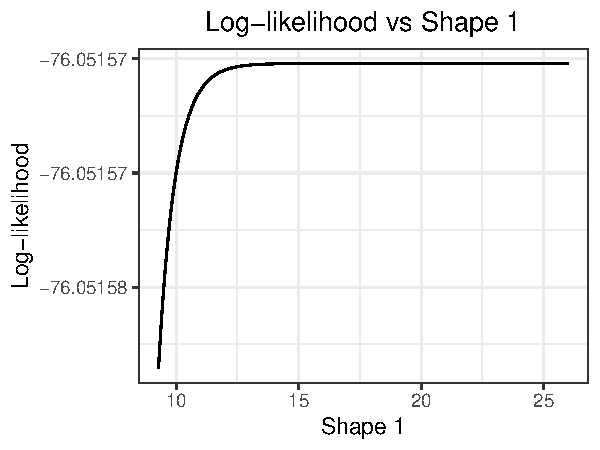
\includegraphics{image/last_plot} 

}

\caption{Log-likelihood profile of a flat surface (non-unique MLE)}\label{fig:flat-loglike-prof}
\end{figure}

We simply made the MTTF of the first component much smaller than the
others, and for even large samples there was not generally enough
information to estimate the parameters of the other components. In this
case, the MLE is not unique, and the likelihood surface is flat, as
shown.

We encountered this issue in our simulation study for small samples due
to right-censored and masked component cause of failure data, despite
parameterizing a series system with components that have similar MTTFs.
Our decision was to simply exclude these data sets from our analysis,
since they are not informative enough to estimate the parameters of the
system.

\textbf{Parameter rescaling}: When the parameters under investigation
span different orders of magnitude, parameter rescaling can
significantly improve the performance and reliability of optimization
algorithms. Parameter rescaling gives an optimizer a sense of the
typical size of each parameter, enabling it to adjust its steps
accordingly. This is crucial in scenarios like ours, where shape and
scale parametes are a few orders of magnitude apart. Without rescaling,
the optimization routine may struggle, taking numerous small steps for
larger parameters and overshooting for smaller ones.

Speed of convergence was particularly important in our case, since in
our simulation study, we employ the Bootstrap method to estimate the
sampling distribution of the MLE, which requires us to estimate the MLE
for many data sets. We found that parameter rescaling significantly
improved the speed of convergence, which allowed us to run our
simulation study in a tractable amount of time.

\hypertarget{simulation-design}{%
\subsection{Simulation Design}\label{simulation-design}}

In this section, we describe the design of our simulation study. We
first describe the simulation scenarios we consider, and then we
describe how we generate data for each scenario.

\hypertarget{bernoulli-candidate-set-model}{%
\subsubsection{Bernoulli Candidate Set
Model}\label{bernoulli-candidate-set-model}}

In our simulation study, we must generate data that satisfies the
masking conditions described in Section \ref{sec:candmod}. There are
many ways to satisfying the masking conditions. We choose the simplest
method, which we call the \emph{Bernoulli candidate set model}. In this
model, each non-failed component is included in the candidate set with a
fixed probability \(p\), independently of all other components and
independently of \(\boldsymbol{\theta}\), and the failed component is
always included in the candidate set.

\hypertarget{right-censoring-model}{%
\subsubsection{Right-Censoring Model}\label{right-censoring-model}}

We employ a very simple right-censoring model, where the right-censoring
time \(\tau\) is fixed and independent of \(\boldsymbol{\theta}\) and
the censoring time \(S_i\) of the \(i\)\textsuperscript{th} system.

We parameterize \(\tau\) by quantiles of the series system, e.g., if
\(q = 0.8\), then \(\tau(q)\) is the \(80\%\) quantile of the series
system such that \(80\%\) of the series systems are observed (fail
before time \(\tau(q)\)) and \(20\%\) of the series systems fail after
time \(\tau(q)\) (are right-censored).

\hypertarget{scenarios}{%
\subsubsection{Scenarios}\label{scenarios}}

we vary the sample size \(n\), the Bernoulli masking probability \(p\)
of including each non-failed component in the candidate set, and the
right-censoring time \(\tau\). We then analyze the performance of the
MLE under these various scenarios.

Here is an outline of the simulation study analysis:

\begin{enumerate}
\def\labelenumi{\arabic{enumi}.}
\item
  Set up simulation parameters for various scenarios of interest, such
  as generating data to examine the relationship between bias and
  masking probability for different sample sizes and right-censoring
  times.
\item
  Generate \(R\) data sets for each scenario (some combination of \(n\),
  \(p\), and \(\tau\)).
\item
  Estimate the parameters for each data set, giving us \(R\) estimates
  of the parameters. We use these data sets as an empirical estimate of
  the sampling distribution of the MLE for each scenario.
\item
  Using the empirical sampling distribution of the MLE, estimate various
  performance measures of the MLE, like bias, variance, MSE, and
  coverage probability for each scenario.
\item
  Analyze and visualize the results, e.g., by plotting the bias,
  variance, MSE, and coverage probability as a function of \(n\) for
  different combinations of \(p\) and \(\tau\).

  We then interpret the results and discuss the performance of the MLE
  estimator under various conditions. We expect that as
  \(n \to \infty\), the bias and MSE will go to \(0\) and the coverage
  probability will go to \(0.95\) (when constructing \(95\%\) confidence
  intervals). Of course, we do not expect these results to hold for
  finite \(n\), but we would like to see how the bias, MSE, and coverage
  probability change as we vary \(n\), \(p\), and \(\tau\).
\end{enumerate}

For how we generate a scenario, see Appendix A.

\begin{quote}
So, now we just resample from the data with replacement, and fit the
Weibull series model to each bootstrap sample. We do this \(B = 1000\)
times, giving us \(B\) bootstrap replicates of the MLE
\(\hat{\boldsymbol{\theta}}^{(1)},\ldots,\hat{\boldsymbol{\theta}}^{(B)}\).
\end{quote}

\begin{quote}
As a ground truth, we will use the empirical distribution of the MLE
under our data model under a variety of simulation scenarios where we
vary the sample size, the right censoring time, and the so-called
masking probability of the candidate sets, where a higher masking
probability means that the candidate sets are more likely to contain
non-failed components.
\end{quote}

\hypertarget{verification}{%
\subsubsection{Verification}\label{verification}}

To verify that our likelihood model is correct, we load the Table 2 data
from \citep{Huairu-2013} and fit the Weibull series model to the data to
see if we can recover the MLE they reported. When we fit the Weibull
series model to this data by maximizing the likelihood function, we
obtain the following fit for the shape and scale parameters given
respectively by \[
    \hat{k}_1 = 1.2576,
    \hat{k}_2 = 1.1635,
    \hat{k}_3 = 1.1308,
\] and \[
    \hat{\lambda}_1 = 994.3661,
    \hat{\lambda}_2 = 908.9458,
    \hat{\lambda}_3 = 840.1141,
\] which is in agreement with the MLE they reported. Satisfied that our
likelihood model is correct, we proceed with the simulation study.

\hypertarget{sec:acc_prec}{%
\subsection{Bias, variance, and MSE of the MLE}\label{sec:acc_prec}}

First, we estimate the bias, variance, and MSE of the MLE under various
scenarios. This is useful for understanding the accuracy and precision
of the MLE under different conditions. It is unrelated to the bootstrap
method, but it is useful to compute these quantities before we assess
the bootstrapped variance and confidence intervals.

A measure of the accuracy of \(\boldsymbol{\hat\theta}\) is the bias,
which is defined as \[
\operatorname{b}(\boldsymbol{\hat\theta}) = E(\boldsymbol{\hat\theta}) - \boldsymbol{\theta}.
\] We cannot analytically derive the bias, so we estimate the bias using
the empirical sampling distribution, \[
\hat{\operatorname{b}}(\hat\theta_j) =
    E_{\hat{\boldsymbol{\theta}} \sim \text{data}}(\boldsymbol{\hat\theta}) - \theta_j.
\]

We estimate the precision of \(\hat\theta_j\) with the variance and MSE.
The variance of \(\boldsymbol{\hat\theta}\) is defined as \[
\operatorname{Var}(\hat\theta_j) =
    E_{\hat{\boldsymbol{\theta}} \sim \text{data}}\bigl((\hat\theta_j - E_{\hat{\boldsymbol{\theta}} \sim \text{data}}(\hat\theta_j))^2\bigr),
\] where the expectation is taken with respect to the empirical sampling
distribution. The mean squared error is a measure of estimator error
that incorporates both the bias and the variance, and is defined as \[
\operatorname{MSE}(\hat\theta_j) =
    E_{\hat{\boldsymbol{\theta}} \sim \text{data}}\bigl((\hat\theta_j - \theta_j)^2\bigr).
\]

Assuming the regularity conditions for the MLE are met, the MSE
converges in probability to the variance.

\hypertarget{simulation-scenarios}{%
\subsection{Simulation Scenarios}\label{simulation-scenarios}}

We consider many different scenarios, where we vary the sample size
\(n\), the masking probability \(p\), and the right-censoring time
\(\tau\). We then analyze the performance of the MLE under these various
scenarios by estimating the bias, variance, and MSE of the MLE.

\hypertarget{absolute-bias-vs.-sample-size-with-a-masking-probability-but-no-right-censoring}{%
\subsubsection*{Absolute bias vs.~sample size with a masking probability
but no
right-censoring}\label{absolute-bias-vs.-sample-size-with-a-masking-probability-but-no-right-censoring}}
\addcontentsline{toc}{subsubsection}{Absolute bias vs.~sample size with
a masking probability but no right-censoring}

In this scenario, we want to see the bias of the MLE as a function of
the sample size \(n\) from \(n = 30\) to \(n = 800\) for a fixed masking
probability \(p = 0.2\) and no right-censoring \((\tau = \infty)\).
Recall that the masking probability is the probability of including each
non-failed component.

\begin{figure}

{\centering 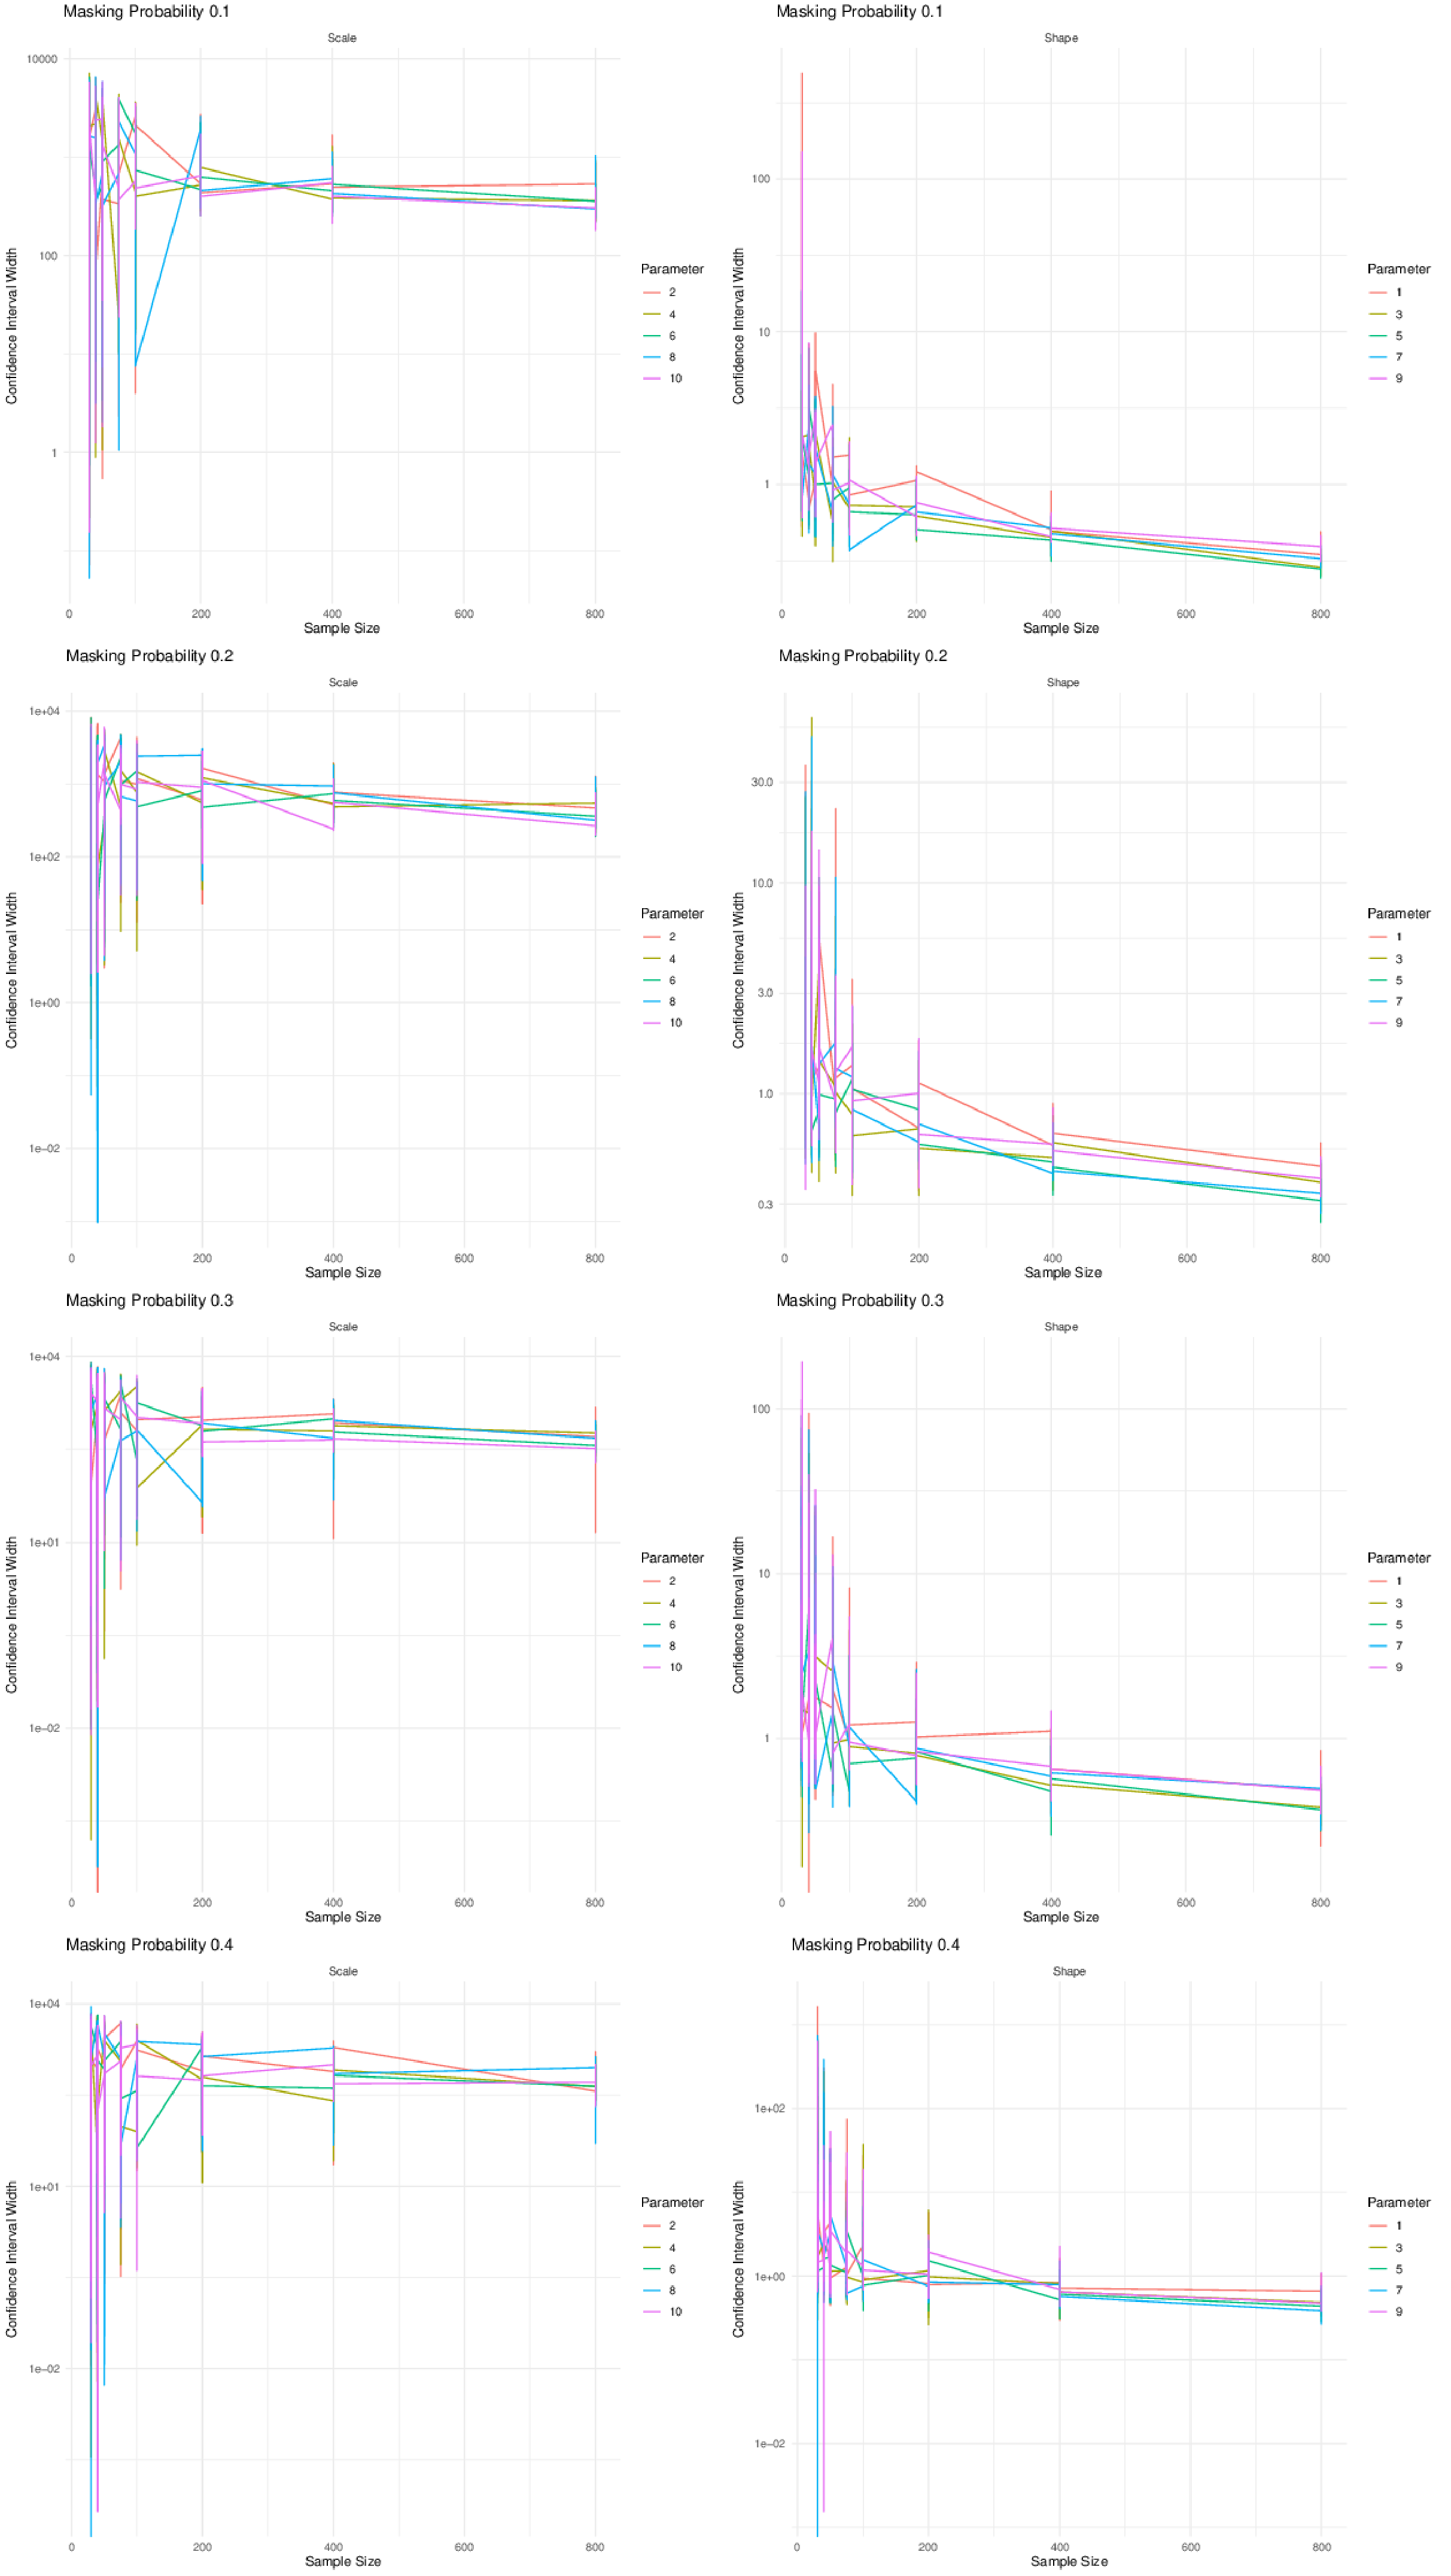
\includegraphics{image/plot-p-0.2-bias-vs-sample-size} 

}

\caption{Bias vs. sample size (masking probability 0.2)}\label{fig:plot-bias-p-0.2-vs-sample-size}
\end{figure}

In Figure \ref{fig:plot-bias-p-0.2-vs-sample-size}, we plot the absolute
bias \(|\operatorname{bias}(\hat\theta)|\) on a log scale against the
sample size. However, because the absolute bias is quite large for small
sample sizes and small for large sample sizes, we use a log scale.
Furthermore, we show the absolute bias for the shape and scale
parameters separately, since the scale parameters are much larger than
the shape parameters.

Here are some important observations Figure
\ref{fig:plot-bias-p-0.2-vs-sample-size} reveals:

\begin{enumerate}
\def\labelenumi{\arabic{enumi}.}
\item
  For both shape and scale parameters, we see that the absolute bias
  seems to be decreasing to zero as the sample size increases. This is
  not surprising since we expect the MLE to be consistent, i.e.,
  \(\boldsymbol{\hat\theta}\) converges in probability to
  \(\boldsymbol{\theta}\) as the sample size increases to infinity.
  Still, it is reassuring to see that the bias seems to be behaving as
  expected.
\item
  For the shape parameters, which are small (the shape parameters have
  true values a little larger than 1), the bias is relatively large for
  sample sizes up to \(100\).
\item
  For the scale parameters, which are quite large (the scale parameters
  have true values around 1000). Like with the shape parameters, the
  bias is relatively large for sample sizes up to \(100\), but seems to
  stabilize and reach relatively small values after that.
\end{enumerate}

\hypertarget{scenario-bias-vs.-sample-size-and-masking-probability-and-no-right-censoring}{%
\subsubsection*{Scenario: Bias vs.~sample size and masking probability
and no
right-censoring}\label{scenario-bias-vs.-sample-size-and-masking-probability-and-no-right-censoring}}
\addcontentsline{toc}{subsubsection}{Scenario: Bias vs.~sample size and
masking probability and no right-censoring}

Now, we take a larger view and plot the bias (without taking its
absolute value as we had done previously) against the masking
probabilities \(p = 0\) (no masking) to \(p = 0.4\) (significant
masking) for sample sizes 100, 400, and 800.

For the shape parameters, at a sample of size 100, we see significant
bias and we also see that it is very sensitive to the masking
probability. See Figure
\ref{fig:plot-bias-shapes-vs-p-sample-size-100-400-800}. However, for
sample sizes of 400 and 800, the bias is relatively small and unaffected
by the masking probability.

\begin{figure}

{\centering 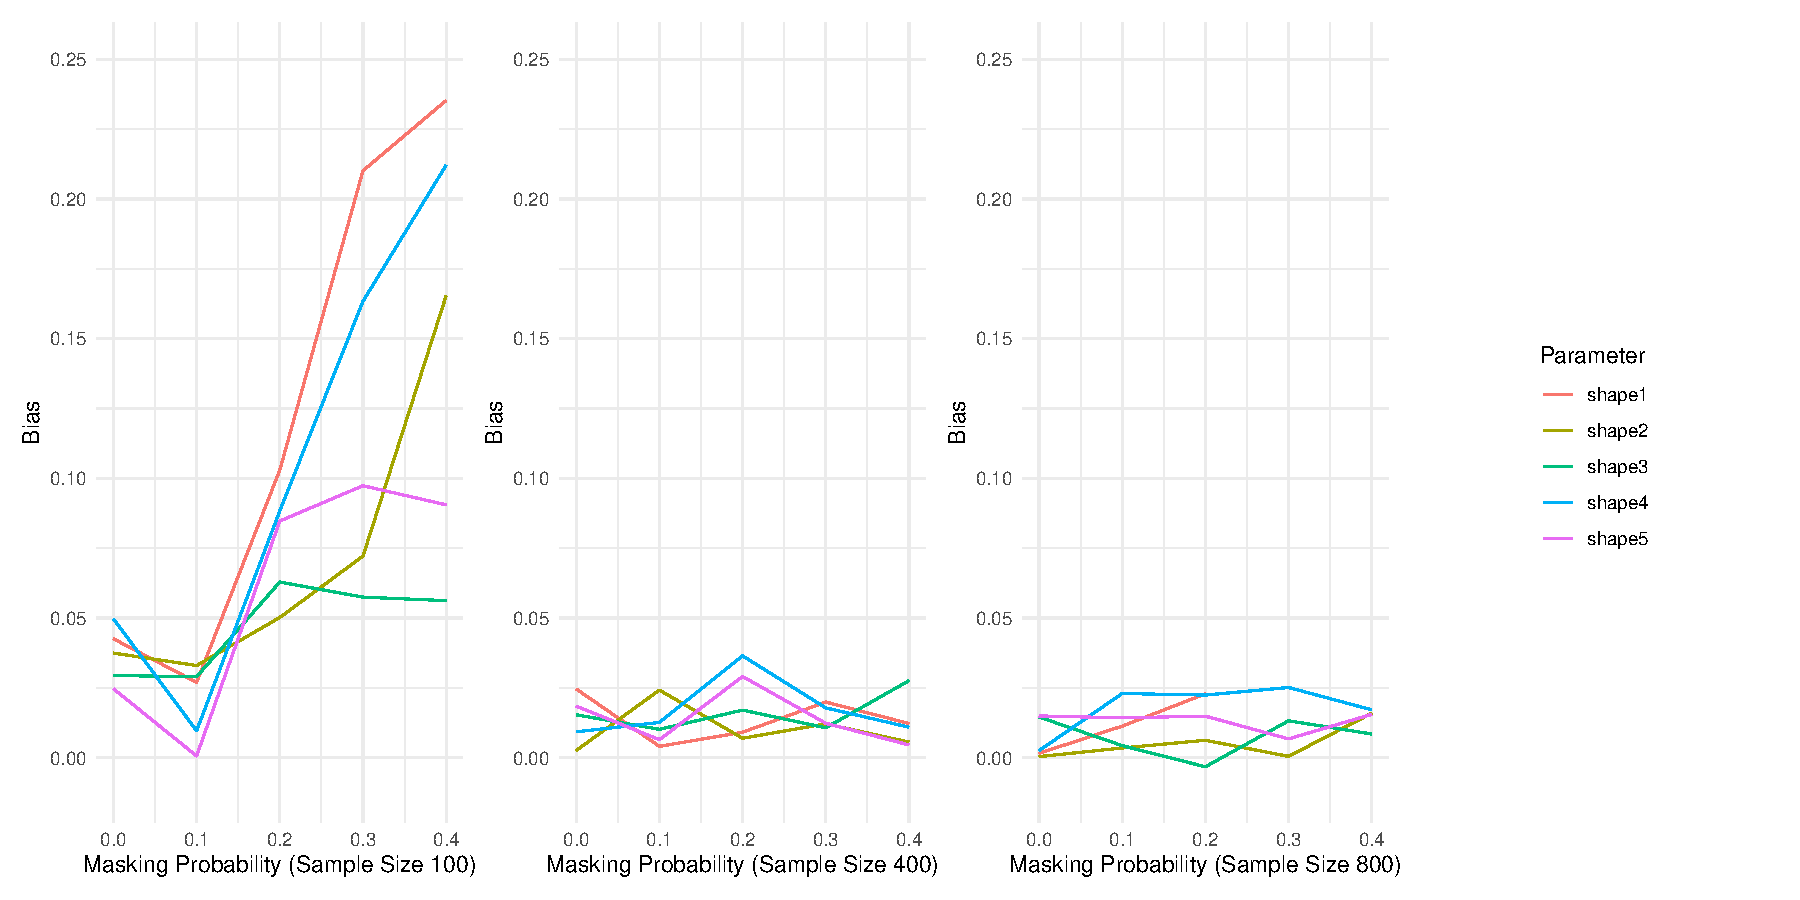
\includegraphics{image/plot-bias-shapes-p-vs-sample-size-100-400-800} 

}

\caption{Shape Bias vs. masking probability for sample sizes 100, 400, and 800}\label{fig:plot-bias-shapes-vs-p-sample-size-100-400-800}
\end{figure}

For the scale parameters, a similar pattern emerges, although we see
that even for sample size 400, there is evidence that the bias is still
affected by the masking probability. See Figure
\ref{fig:plot-bias-scales-vs-p-sample-size-100-400-800}.

The smallest bias, as expected, occurs for sample sizes of \(800\). The
bias for \(\lambda_1\) (scale parameter 1) at the masking probability
\(0.3\) is an interesting case, since it jumps up at that point for some
reason. We used only \(R = 100\) replications, so it is plausible it
would decrease with more replications. Regardless, the overall trend is
that the bias decreases as the sample size increases, and its dependence
on the masking probability is relatively small with sufficiently large
sample sizes.

\begin{figure}

{\centering 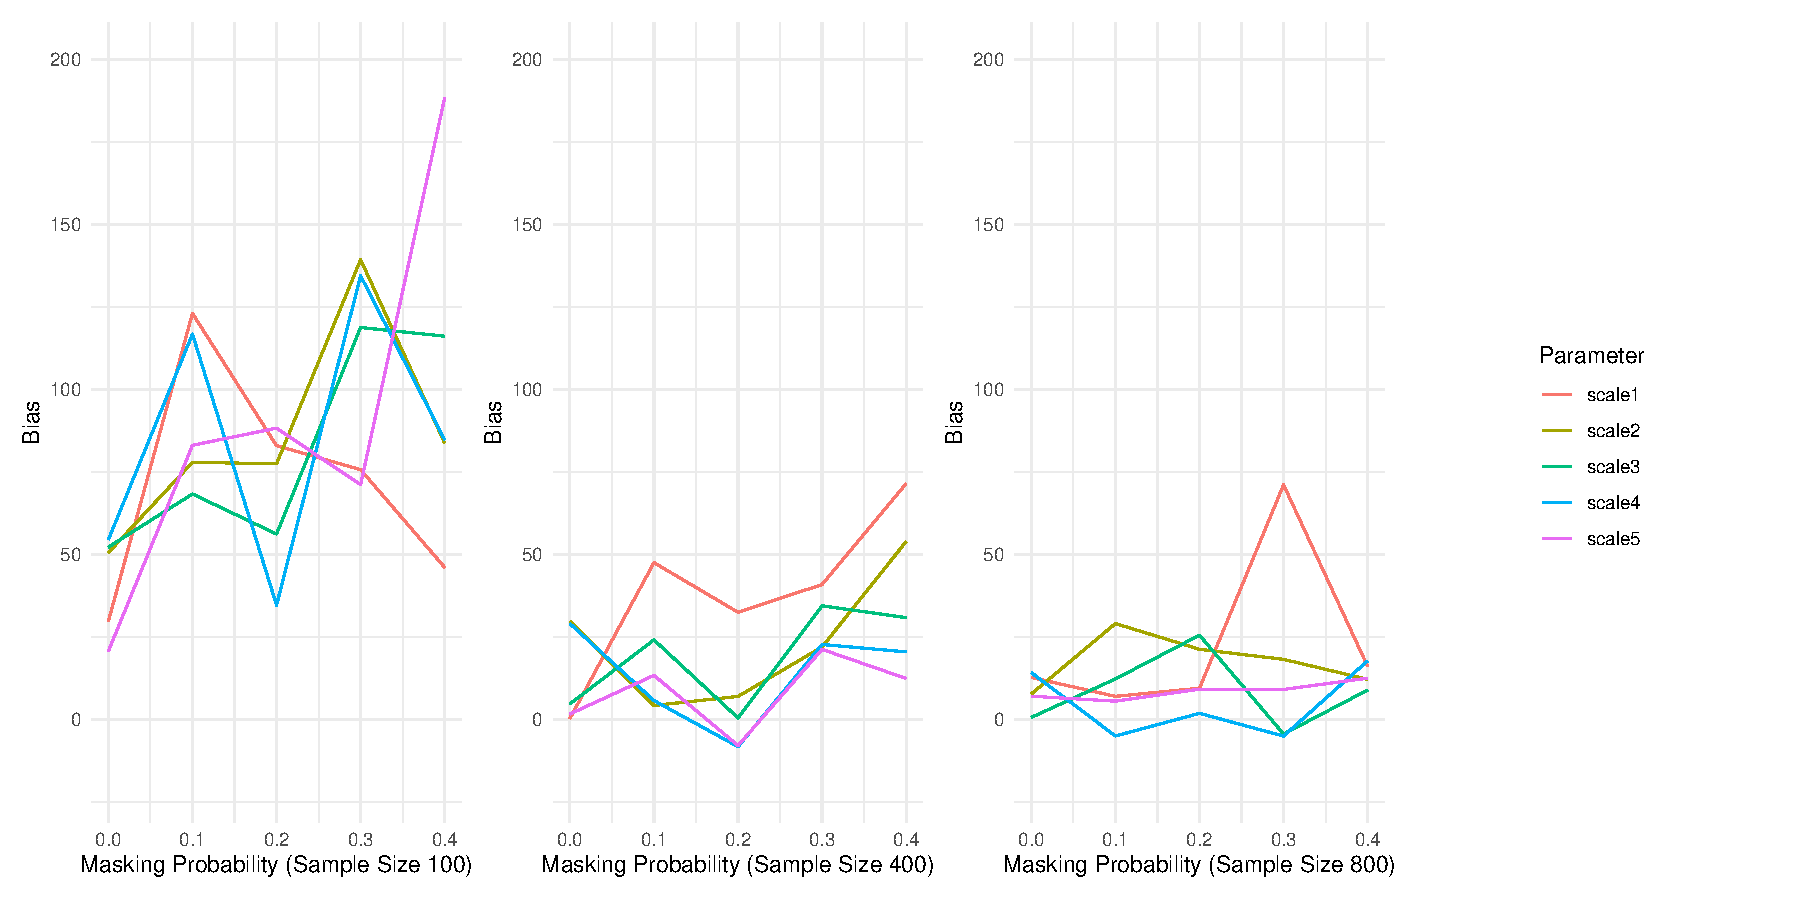
\includegraphics{image/plot-bias-scales-p-vs-sample-size-100-400-800} 

}

\caption{Scale Bias vs. masking probability for sample sizes 100, 400, and 800}\label{fig:plot-bias-scales-vs-p-sample-size-100-400-800}
\end{figure}

\hypertarget{scenario-bias-vs.-right-censoring-time-and-sample-size-with-a-fixed-masking-probability}{%
\paragraph*{Scenario: Bias vs.~right-censoring time and sample size with
a fixed masking
probability}\label{scenario-bias-vs.-right-censoring-time-and-sample-size-with-a-fixed-masking-probability}}
\addcontentsline{toc}{paragraph}{Scenario: Bias vs.~right-censoring time
and sample size with a fixed masking probability}

In this scenario, we want to isolate the effect of the right-censoring
time \(\tau\) on the bias. We fix the masking probability to
\(p = 0.215\), in line with the masking probability we estimate for the
Table 2 data set in \citep{Huairu-2013}.

We plot the bias against the right-censoring time for sample sizes 50,
150, and 300. See Figure
\ref{fig:plot-bias-tau-vs-sample-size-50-150-300}. On the \(x\)-axis, we
report the right-censoring time as a quantile of the Weibull series
distribution so that we can more clearly see the effect of the
right-censoring on the bias, e.g., the \(50\%\) quantile is the time at
which \(50\%\) of the systems are expected to fail.

\begin{figure}

{\centering 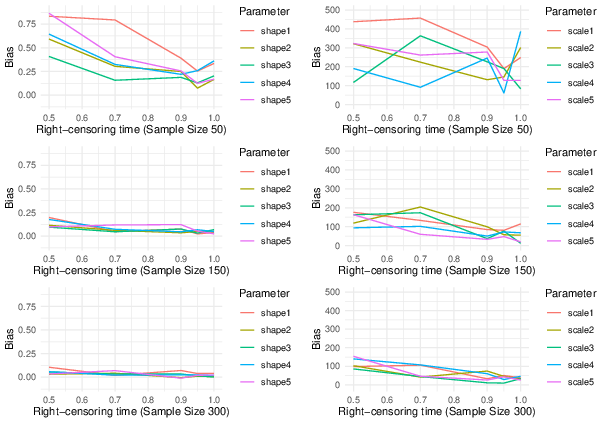
\includegraphics{image/plot-bias-tau-vs-sample-size-50-150-300} 

}

\caption{Bias vs. right-censoring time and sample sizes 50, 150, and 300}\label{fig:plot-bias-tau-vs-sample-size-50-150-300}
\end{figure}

A few observations about Figure
\ref{fig:plot-bias-tau-vs-sample-size-50-150-300}:

\begin{enumerate}
\def\labelenumi{\arabic{enumi}.}
\item
  The bias decreases as the right-censoring time increases. This is
  expected since we have more information about the system when the
  right-censoring time is larger.
\item
  The bias decreases as the sample size increases, which is also
  expected since we have more information about the system when the
  sample size is larger.
\item
  The bias is relatively small for sample sizes 150 and 300, but for
  sample size 50, the bias is quite large, particularly for the shape
  parameters. This is not surprising since the sample size is quite
  small, and so we do not expect the MLE to be very accurate.
\end{enumerate}

\hypertarget{variance}{%
\subsubsection{Variance}\label{variance}}

\begin{verbatim}
## -- Attaching core tidyverse packages ------------------------ tidyverse 2.0.0 --
## v forcats   1.0.0     v stringr   1.5.0
## v lubridate 1.9.2     v tibble    3.2.1
## v purrr     1.0.1     v tidyr     1.3.0
## -- Conflicts ------------------------------------------ tidyverse_conflicts() --
## x gridExtra::combine() masks dplyr::combine()
## x dplyr::filter()      masks stats::filter()
## x dplyr::lag()         masks stats::lag()
## i Use the conflicted package (<http://conflicted.r-lib.org/>) to force all conflicts to become errors
\end{verbatim}

\begin{verbatim}
## Warning: One or more parsing issues, call `problems()` on your data frame for details,
## e.g.:
##   dat <- vroom(...)
##   problems(dat)
\end{verbatim}

\begin{verbatim}
## Rows: 64000 Columns: 54
## -- Column specification --------------------------------------------------------
## Delimiter: ","
## chr (10): coverages.1, coverages.2, coverages.3, coverages.4, coverages.5, c...
## dbl (44): n, p, q, tau, mle.1, mle.2, mle.3, mle.4, mle.5, mle.6, mle.7, mle...
## 
## i Use `spec()` to retrieve the full column specification for this data.
## i Specify the column types or set `show_col_types = FALSE` to quiet this message.
\end{verbatim}

\begin{figure}

{\centering 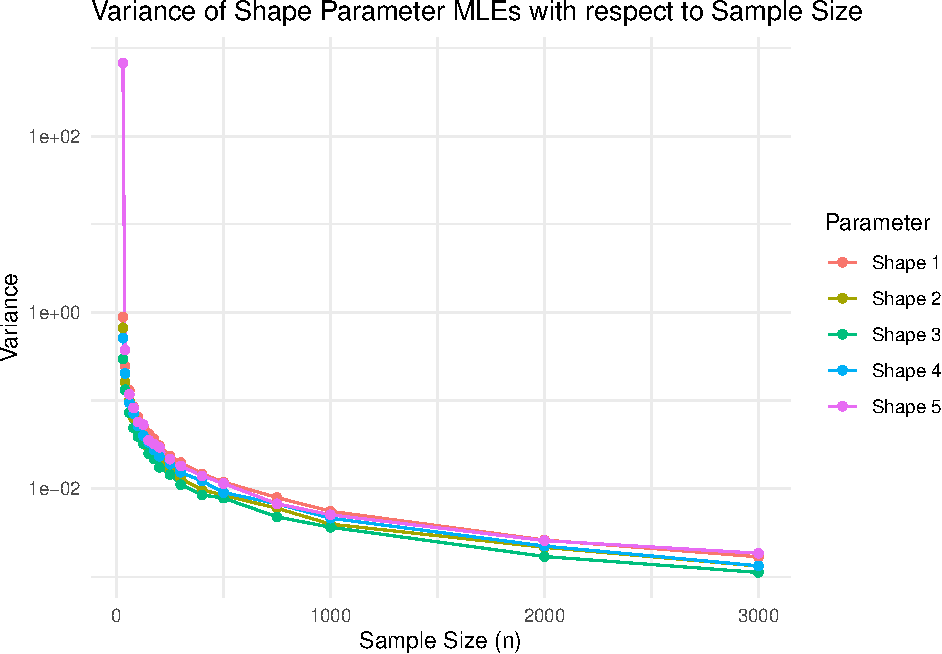
\includegraphics{wei_series_md_files/figure-latex/var.plot-1} 

}

\caption{Variance vs. sample size}\label{fig:var.plot-1}
\end{figure}
\begin{figure}

{\centering 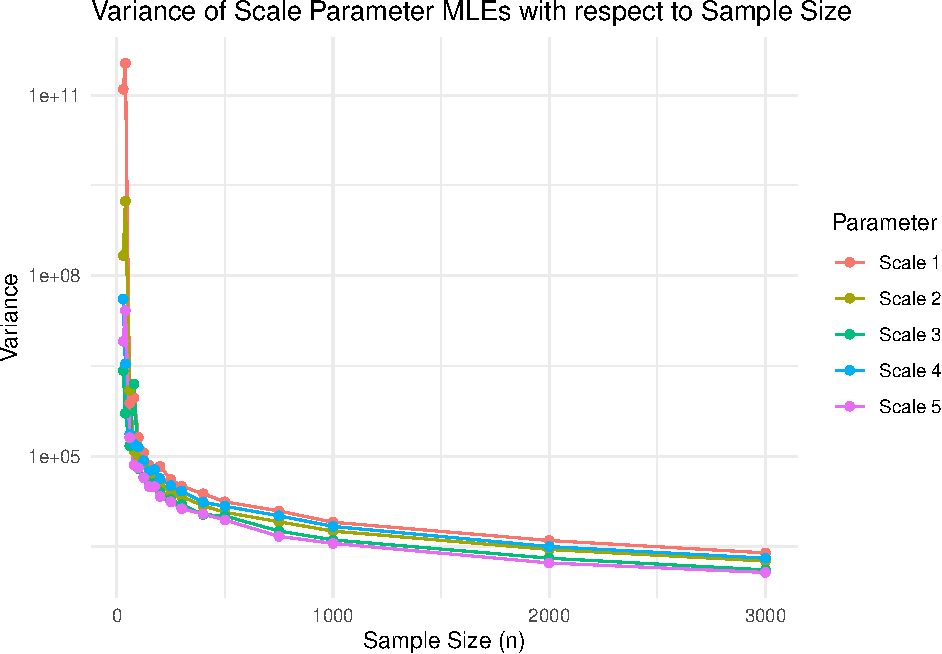
\includegraphics{wei_series_md_files/figure-latex/var.plot-2} 

}

\caption{Variance vs. sample size}\label{fig:var.plot-2}
\end{figure}

\hypertarget{sec:coverage_prob}{%
\subsection{Coverage Probability of Bootstrapped Confidence
Intervals}\label{sec:coverage_prob}}

Under a variety of scenarios, we will bootstrap a \(95\%\)-confidence
interval for \(\boldsymbol{\theta}\) using the percentile method, and we
will evaluate its accuracy by computing the coverage probability.

We want the coverage probability to be close to the nominal level,
\(95\%\), because if the coverage probability is too low, then we will
be too confident in the precision and accuracy of the MLE, and if the
coverage probability is too high, then we will not be confident enough
in the precision and accuracy of the MLE.

To estimate the coverage probability, we use the following procedure:

\begin{enumerate}
\def\labelenumi{\arabic{enumi}.}
\item
  For a given scenario, we generate \(R = 300\) data sets.
\item
  We find an MLE for each of \(R\) data sets.
\item
  We bootstrap the \(95\%\)-confidence interval for each MLE.
\item
  We compute the coverage probability by computing the proportion of
  times the true parameter \(\boldsymbol{\theta}\) is contained in
  \(95\%\)-confidence interval.
\end{enumerate}

\hypertarget{simulation-scenarios-1}{%
\subsection{Simulation Scenarios}\label{simulation-scenarios-1}}

\hypertarget{scenario-coverage-probability-vs.-sample-size-with-a-fixed-masking-probability-and-no-right-censoring}{%
\subsubsection*{Scenario: Coverage probability vs.~sample size with a
fixed masking probability and no
right-censoring}\label{scenario-coverage-probability-vs.-sample-size-with-a-fixed-masking-probability-and-no-right-censoring}}
\addcontentsline{toc}{subsubsection}{Scenario: Coverage probability
vs.~sample size with a fixed masking probability and no right-censoring}

We want to isolate the effect of the coverage probability as a function
of the sample size \(n\). We fix the masking probability to \(p = 0.2\)
and without right-censoring \((\tau = \infty)\) and vary the sample size
from \(n = 30\) to \(n = 800\). See Figure
\ref{fig:plot-coverage-p-three-vs-sample-size}.

\begin{figure}

{\centering 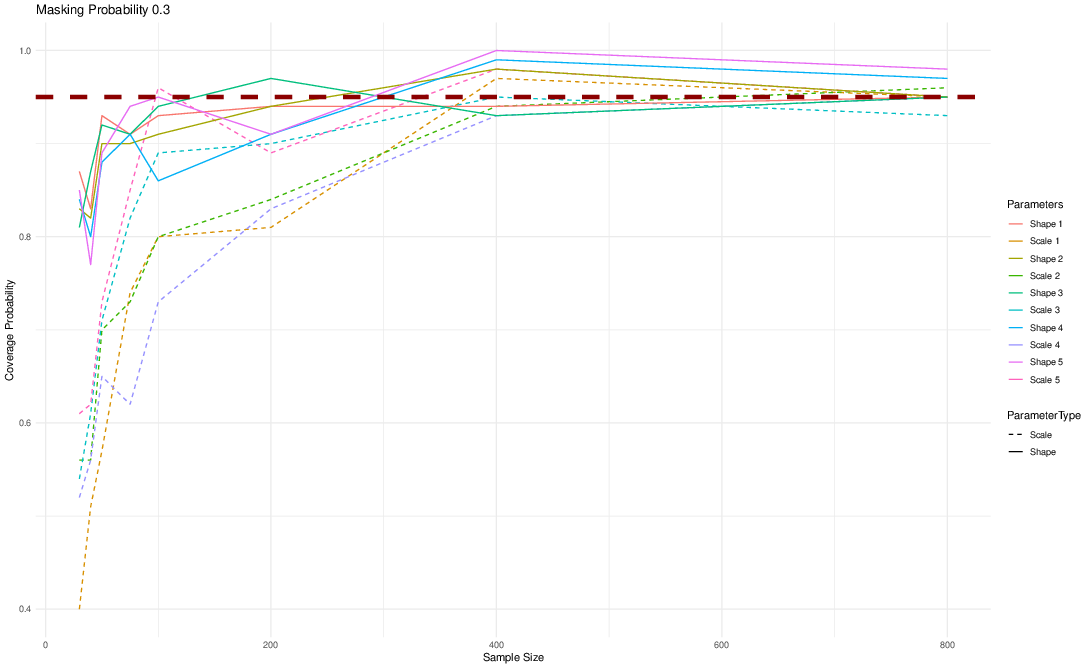
\includegraphics{image/plot-coverage-p_0.3-vs-sample-size} 

}

\caption{Coverage probability vs. sample size for masking probability $0.3$}\label{fig:plot-coverage-p-three-vs-sample-size}
\end{figure}

Here are some key observations:

\begin{enumerate}
\def\labelenumi{\arabic{enumi}.}
\item
  It is immediately obvious that the scale parameters (dashed lines)
  have a much lower coverage probability than the shape parameters
  (solid lines), particularly for small sample sizes less than
  \(n = 200\).

  In general, the scale parameters appear to be more difficult to
  estimate than the shape parameters.
\item
  As the sample size increases, the coverage probability for the shape
  parameters and scale parameters approaches the nominal level,
  \(95\%\).

  This suggests that the sampling distribution of the MLE is converging
  in distribution to a multivariate normal distribution with mean
  \(\boldsymbol{\theta}\) and variance-covariance given by the inverse
  of the FIM, consistent with the asymptotic theory.
\end{enumerate}

\hypertarget{scenario-coverage-probability-vs.-sample-size-and-masking-probability-without-right-censoring}{%
\subsubsection*{Scenario: Coverage probability vs.~sample size and
masking probability without
right-censoring}\label{scenario-coverage-probability-vs.-sample-size-and-masking-probability-without-right-censoring}}
\addcontentsline{toc}{subsubsection}{Scenario: Coverage probability
vs.~sample size and masking probability without right-censoring}

We want to get a larger picture of how the coverage probability depends
on the sample size \(n\) and masking probability \(p\). We fix the
right-censoring time to \(\tau = \infty\) and vary the sample size from
\(n = 30\) to \(n = 800\) and vary the masking probability from
\(p = 0\) (no masking) to \(p = 0.4\) and then compute the coverage
probability for each combination of sample size \(n\) and masking
probability \(p\).

\begin{figure}

{\centering 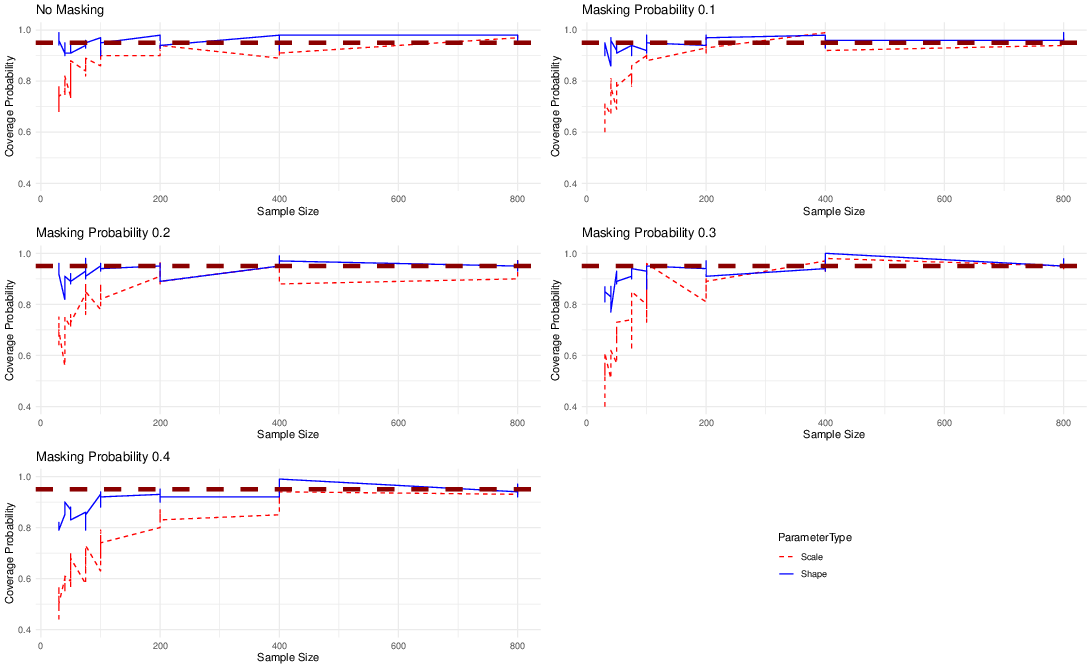
\includegraphics{image/plot-coverage-p-vs-sample-size} 

}

\caption{Coverage probability vs. sample size}\label{fig:plot-coverage-p-vs-sample-size}
\end{figure}

The results of this analysis are summarized by Figure
\ref{fig:plot-coverage-p-vs-sample-size}. Here are some key
observations:

\begin{enumerate}
\def\labelenumi{\arabic{enumi}.}
\item
  For sample sizes \(n \leq 100\), the coverage probability for the
  shape parameters is close to the nominal level, \(95\%\), only for
  small masking probabilities. However, as the sample size increases,
  the coverage probability for the shape parameters quickly approaches
  the nominal level, \(95\%\), for all masking probabilities reported
  here.
\item
  For the scale parameters, the coverage probability is too low for all
  sample sizes \(n < 200\) for all masking probabilities reported here.
  For small sample sizes, the confience intervals particularly for the
  scale parameters, should probably be taken with a grain of salt.
\end{enumerate}

In Section \ref{sec:boot}, we explore an alternative way to construct
confidence intervals using the bootstrap method, which is generally a
more accurate way to compute confidence intervals. Unlike the inverse of
the observed FIM, it does not assume that the sampling distribution of
the MLE is asymptotically normal, and so it is more robust to violations
of this assumption.

\hypertarget{conclusion}{%
\section{Conclusion}\label{conclusion}}

We have developed a likelihood model for series systems with latent
components and right-censoring. We have provided evidence that, as long
as certain regularity conditions are met, the MLE is asymptotically
unbiased and consistent.

\hypertarget{references}{%
\section*{References}\label{references}}
\addcontentsline{toc}{section}{References}

Please see below for a full list of references.

\hypertarget{refs}{}
\begin{cslreferences}
\end{cslreferences}

\hypertarget{app}{%
\section{Appendix}\label{app}}

\hypertarget{app:data}{%
\subsection{Data}\label{app:data}}

\hypertarget{simulation-code}{%
\subsection*{Simulation Code}\label{simulation-code}}
\addcontentsline{toc}{subsection}{Simulation Code}

\begin{Shaded}
\begin{Highlighting}[]
\CommentTok{\#\#\#\#\#\#\#\#\#\#\#\#\#\#\#\#\#\#\#\#\#\#\#\#\#\#\#\#\#\#\#\#\#\#\#\#\#\#\#\#\#\#\#\#\#\#\#\#\#\#\#\#\#\#\#\#\#\#\#\#\#}
\CommentTok{\# Simulation data generating process for specified scenario \#}
\CommentTok{\# (n, p, q), where:                                         \#}
\CommentTok{\#    {-} n is a vector of sample sizes                        \#}
\CommentTok{\#     {-} n is a vector of sample sizes                       \#}
\CommentTok{\#     {-} p is a vector of masking probabilities              \#}
\CommentTok{\#     {-} q is a vector of right{-}censoring quantiles of the   \#}
\CommentTok{\#       Weibull series distribution.                        \#}
\CommentTok{\#\#\#\#\#\#\#\#\#\#\#\#\#\#\#\#\#\#\#\#\#\#\#\#\#\#\#\#\#\#\#\#\#\#\#\#\#\#\#\#\#\#\#\#\#\#\#\#\#\#\#\#\#\#\#\#\#\#\#\#\#}

\CommentTok{\# here is the R libary we developed for this project}
\KeywordTok{library}\NormalTok{(wei.series.md.c1.c2.c3) }

\CommentTok{\# for parallel processing}
\KeywordTok{library}\NormalTok{(parallel)}

\CommentTok{\# you can set a seed for reproducibility of the experimental run}
\CommentTok{\# however, if you use parallel processing, this simple approach will not work.}
\CommentTok{\# set.seed(1234)}

\CommentTok{\#\#\#\#\#\#\#\#\#\#\#\#\#\#\#\#\#\#\#\#\#\#\#\#\#\#\#\#\#\#\#\#\#\#\#\#\#\#\#\#\#\#\#\#\#\#\#}
\CommentTok{\# Here is an example of how to run a scenario \#}
\CommentTok{\#\#\#\#\#\#\#\#\#\#\#\#\#\#\#\#\#\#\#\#\#\#\#\#\#\#\#\#\#\#\#\#\#\#\#\#\#\#\#\#\#\#\#\#\#\#\#}

\CommentTok{\# set the simulation name to be used in the file names}
\NormalTok{sim.name \textless{}{-}}\StringTok{ "sim{-}2"}
\CommentTok{\# set the sample sizes}
\NormalTok{ns \textless{}{-}}\StringTok{ }\KeywordTok{c}\NormalTok{(}\DecValTok{30}\NormalTok{, }\DecValTok{40}\NormalTok{, }\DecValTok{50}\NormalTok{, }\DecValTok{75}\NormalTok{, }\DecValTok{100}\NormalTok{, }\DecValTok{200}\NormalTok{, }\DecValTok{400}\NormalTok{, }\DecValTok{800}\NormalTok{)}
\CommentTok{\# set the masking probabilities}
\NormalTok{ps \textless{}{-}}\StringTok{ }\KeywordTok{seq}\NormalTok{(}\DecValTok{0}\NormalTok{, }\DecValTok{0}\NormalTok{,}\DecValTok{1}\NormalTok{, }\FloatTok{0.2}\NormalTok{, }\FloatTok{0.3}\NormalTok{, }\FloatTok{0.4}\NormalTok{)}
\CommentTok{\# set the right{-}censoring quantiles}
\NormalTok{qs \textless{}{-}}\StringTok{ }\KeywordTok{c}\NormalTok{(}\FloatTok{0.5}\NormalTok{, }\FloatTok{0.6}\NormalTok{, }\FloatTok{0.7}\NormalTok{, }\FloatTok{0.8}\NormalTok{, }\FloatTok{0.9}\NormalTok{, }\FloatTok{0.95}\NormalTok{)}
\CommentTok{\# set the number of replicates}
\NormalTok{R \textless{}{-}}\StringTok{ }\DecValTok{100}
\CommentTok{\# set the number of CPU cores to use}
\NormalTok{ncores \textless{}{-}}\StringTok{ }\DecValTok{4}

\CommentTok{\# true parameter values}
\NormalTok{theta \textless{}{-}}\StringTok{ }\KeywordTok{c}\NormalTok{(}\DataTypeTok{shape1 =} \FloatTok{1.2576}\NormalTok{, }\DataTypeTok{scale1 =} \FloatTok{994.3661}\NormalTok{,}
           \DataTypeTok{shape2 =} \FloatTok{1.1635}\NormalTok{, }\DataTypeTok{scale2 =} \FloatTok{908.9458}\NormalTok{,}
           \DataTypeTok{shape3 =} \FloatTok{1.1308}\NormalTok{, }\DataTypeTok{scale3 =} \FloatTok{840.1141}\NormalTok{,}
           \DataTypeTok{shape4 =} \FloatTok{1.1802}\NormalTok{, }\DataTypeTok{scale4 =} \FloatTok{940.1141}\NormalTok{,}
           \DataTypeTok{shape5 =} \FloatTok{1.3311}\NormalTok{, }\DataTypeTok{scale5 =} \FloatTok{836.1123}\NormalTok{)}

\NormalTok{shapes \textless{}{-}}\StringTok{ }\NormalTok{theta[}\KeywordTok{seq}\NormalTok{(}\DecValTok{1}\NormalTok{, }\KeywordTok{length}\NormalTok{(theta), }\DecValTok{2}\NormalTok{)]}
\NormalTok{scales \textless{}{-}}\StringTok{ }\NormalTok{theta[}\KeywordTok{seq}\NormalTok{(}\DecValTok{2}\NormalTok{, }\KeywordTok{length}\NormalTok{(theta), }\DecValTok{2}\NormalTok{)]}

\CommentTok{\# helps the MLE optimization routine converge more quickly and reliably}
\CommentTok{\# by scaling the parameters to be of similar magnitude}
\NormalTok{parscale \textless{}{-}}\StringTok{ }\KeywordTok{c}\NormalTok{(}\DecValTok{1}\NormalTok{, }\DecValTok{1000}\NormalTok{, }\DecValTok{1}\NormalTok{, }\DecValTok{1000}\NormalTok{, }\DecValTok{1}\NormalTok{, }\DecValTok{1000}\NormalTok{, }\DecValTok{1}\NormalTok{, }\DecValTok{1000}\NormalTok{, }\DecValTok{1}\NormalTok{, }\DecValTok{1000}\NormalTok{)}

\NormalTok{sim.run \textless{}{-}}\StringTok{ }\ControlFlowTok{function}\NormalTok{(sim.name, n, p, q, }\DataTypeTok{R =} \DecValTok{1000}\NormalTok{) \{}
\NormalTok{    mles \textless{}{-}}\StringTok{ }\KeywordTok{list}\NormalTok{()}
\NormalTok{    problems \textless{}{-}}\StringTok{ }\KeywordTok{list}\NormalTok{()}

\NormalTok{    tau \textless{}{-}}\StringTok{ }\NormalTok{wei.series.md.c1.c2.c3}\OperatorTok{::}\KeywordTok{qwei\_series}\NormalTok{(}
        \DataTypeTok{p =}\NormalTok{ q, }\DataTypeTok{scales =}\NormalTok{ scales, }\DataTypeTok{shapes =}\NormalTok{ shapes)}

    \KeywordTok{cat}\NormalTok{(}\StringTok{"n ="}\NormalTok{, n, }\StringTok{", p ="}\NormalTok{, p, }\StringTok{", q = "}\NormalTok{, q, }\StringTok{", tau = "}\NormalTok{, tau, }\StringTok{"}\CharTok{\textbackslash{}n}\StringTok{"}\NormalTok{)}

    \ControlFlowTok{for}\NormalTok{ (r }\ControlFlowTok{in} \DecValTok{1}\OperatorTok{:}\NormalTok{R) \{}
\NormalTok{        result \textless{}{-}}\StringTok{ }\KeywordTok{tryCatch}\NormalTok{(\{}

\NormalTok{            df \textless{}{-}}\StringTok{ }\NormalTok{wei.series.md.c1.c2.c3}\OperatorTok{::}\KeywordTok{generate\_guo\_weibull\_table\_2\_data}\NormalTok{(}
                \DataTypeTok{shapes =}\NormalTok{ shapes,}
                \DataTypeTok{scales =}\NormalTok{ scales,}
                \DataTypeTok{n =}\NormalTok{ n,}
                \DataTypeTok{p =}\NormalTok{ p,}
                \DataTypeTok{tau =}\NormalTok{ tau)}

\NormalTok{            sol \textless{}{-}}\StringTok{ }\NormalTok{wei.series.md.c1.c2.c3}\OperatorTok{::}\KeywordTok{mle\_nelder\_wei\_series\_md\_c1\_c2\_c3}\NormalTok{(}
                \DataTypeTok{df =}\NormalTok{ df,}
                \DataTypeTok{theta0 =}\NormalTok{ theta,}
                \DataTypeTok{reltol =} \FloatTok{1e{-}7}\NormalTok{,}
                \DataTypeTok{parscale =}\NormalTok{ parscale,}
                \DataTypeTok{maxit =}\NormalTok{ 2000L)}
\NormalTok{            mles \textless{}{-}}\StringTok{ }\KeywordTok{append}\NormalTok{(mles, }\KeywordTok{list}\NormalTok{(sol))}

            \ControlFlowTok{if}\NormalTok{ (r }\OperatorTok{\%\%}\StringTok{ }\DecValTok{10} \OperatorTok{==}\StringTok{ }\DecValTok{0}\NormalTok{) \{}
                \KeywordTok{cat}\NormalTok{(}\StringTok{"r = "}\NormalTok{, r, }\StringTok{": "}\NormalTok{, sol}\OperatorTok{$}\NormalTok{par, }\StringTok{"}\CharTok{\textbackslash{}n}\StringTok{"}\NormalTok{)}
\NormalTok{            \}}

\NormalTok{        \}, }\DataTypeTok{error =} \ControlFlowTok{function}\NormalTok{(e) \{}
            \KeywordTok{cat}\NormalTok{(}\StringTok{"Error at iteration"}\NormalTok{, r, }\StringTok{":"}\NormalTok{)}
            \KeywordTok{print}\NormalTok{(e)}
\NormalTok{            problems \textless{}{-}}\StringTok{ }\KeywordTok{append}\NormalTok{(problems, }\KeywordTok{list}\NormalTok{(}\KeywordTok{list}\NormalTok{(}
                \DataTypeTok{error =}\NormalTok{ e, }\DataTypeTok{n =}\NormalTok{ n, }\DataTypeTok{p =}\NormalTok{ p, }\DataTypeTok{q =}\NormalTok{ q, }\DataTypeTok{tau =}\NormalTok{ tau, }\DataTypeTok{df =}\NormalTok{ df)))}
\NormalTok{        \})}
\NormalTok{    \}}
  
    \ControlFlowTok{if}\NormalTok{ (}\KeywordTok{length}\NormalTok{(mles) }\OperatorTok{!=}\StringTok{ }\DecValTok{0}\NormalTok{) \{}
        \KeywordTok{saveRDS}\NormalTok{(}\KeywordTok{list}\NormalTok{(}\DataTypeTok{n =}\NormalTok{ n, }\DataTypeTok{p =}\NormalTok{ p, }\DataTypeTok{q =}\NormalTok{ q, }\DataTypeTok{tau =}\NormalTok{ tau, }\DataTypeTok{mles =}\NormalTok{ mles),}
            \DataTypeTok{file =} \KeywordTok{paste0}\NormalTok{(}\StringTok{"./results/"}\NormalTok{, sim.name, }\StringTok{"/results\_"}\NormalTok{, n, }\StringTok{"\_"}\NormalTok{, p, }\StringTok{"\_"}\NormalTok{, q, }\StringTok{".rds"}\NormalTok{))}
\NormalTok{    \}}

    \ControlFlowTok{if}\NormalTok{ (}\KeywordTok{length}\NormalTok{(problems) }\OperatorTok{!=}\StringTok{ }\DecValTok{0}\NormalTok{) \{}
        \KeywordTok{saveRDS}\NormalTok{(}\KeywordTok{list}\NormalTok{(}\DataTypeTok{n =}\NormalTok{ n, }\DataTypeTok{p =}\NormalTok{ p, }\DataTypeTok{q =}\NormalTok{ q, }\DataTypeTok{tau =}\NormalTok{ tau, }\DataTypeTok{problems =}\NormalTok{ problems),}
            \DataTypeTok{file =} \KeywordTok{paste0}\NormalTok{(}\StringTok{"./problems/"}\NormalTok{, sim.name, }\StringTok{"/problems\_"}\NormalTok{, n, }\StringTok{"\_"}\NormalTok{, p, }\StringTok{"\_"}\NormalTok{, q, }\StringTok{".rds"}\NormalTok{))}
\NormalTok{    \}}
\NormalTok{\}}

\NormalTok{params \textless{}{-}}\StringTok{ }\KeywordTok{expand.grid}\NormalTok{(}\DataTypeTok{n =}\NormalTok{ ns, }\DataTypeTok{p =}\NormalTok{ ps, }\DataTypeTok{q =}\NormalTok{ qs)}
\NormalTok{result \textless{}{-}}\StringTok{ }\KeywordTok{mclapply}\NormalTok{(}
    \DecValTok{1}\OperatorTok{:}\KeywordTok{nrow}\NormalTok{(params),}
    \ControlFlowTok{function}\NormalTok{(i) }\KeywordTok{sim.run}\NormalTok{(sim.name, params}\OperatorTok{$}\NormalTok{n[i], params}\OperatorTok{$}\NormalTok{p[i], params}\OperatorTok{$}\NormalTok{q[i], R),}
    \DataTypeTok{mc.cores =}\NormalTok{ ncores)}
\end{Highlighting}
\end{Shaded}

\hypertarget{appendix-b-simulation-of-scenarios-using-the-bootstrap-method}{%
\subsection*{Appendix B: Simulation of scenarios using the Bootstrap
method}\label{appendix-b-simulation-of-scenarios-using-the-bootstrap-method}}
\addcontentsline{toc}{subsection}{Appendix B: Simulation of scenarios
using the Bootstrap method}

\begin{Shaded}
\begin{Highlighting}[]
\CommentTok{\#\#\#\#\#\#\#\#\#\#\#\#\#\#\#\#\#\#\#\#\#\#\#\#\#\#\#\#\#\#\#\#\#\#\#\#\#\#\#\#\#\#\#\#\#\#\#\#\#\#\#\#\#\#\#\#\#\#\#\#\#}
\CommentTok{\# in this scenario, we want to see how we can use the bootstrap}
\CommentTok{\# method to estimate the confidence intervals more precisely (better calibration}
\CommentTok{\# of confidence intervals) for small sample sizes.}
\CommentTok{\# we\textquotesingle{}ll use it to construct a 95\% confidence interval for the estimator. we\textquotesingle{}ll}
\CommentTok{\# compare this result to the asymptotic theory confidence interval.}
\CommentTok{\# finally, we\textquotesingle{}ll generate CIs by each method, asymptotic (inverse FIM) and }
\CommentTok{\# bootstrap (cov), and compare the coverage probabilities.}
\CommentTok{\#\#\#\#\#\#\#\#\#\#\#\#\#\#\#\#\#\#\#\#\#\#\#\#\#\#\#\#\#\#\#\#\#\#\#\#\#\#\#\#\#\#\#\#\#\#\#\#\#\#\#\#\#\#\#\#\#\#\#\#\#}

\KeywordTok{library}\NormalTok{(boot)}
\KeywordTok{library}\NormalTok{(parallel)}
\KeywordTok{library}\NormalTok{(wei.series.md.c1.c2.c3)}

\NormalTok{theta \textless{}{-}}\StringTok{ }\KeywordTok{c}\NormalTok{(}\DataTypeTok{shape1 =} \FloatTok{1.2576}\NormalTok{, }\DataTypeTok{scale1 =} \FloatTok{994.3661}\NormalTok{,}
           \DataTypeTok{shape2 =} \FloatTok{1.1635}\NormalTok{, }\DataTypeTok{scale2 =} \FloatTok{908.9458}\NormalTok{,}
           \DataTypeTok{shape3 =} \FloatTok{1.1308}\NormalTok{, }\DataTypeTok{scale3 =} \FloatTok{840.1141}\NormalTok{,}
           \DataTypeTok{shape4 =} \FloatTok{1.1802}\NormalTok{, }\DataTypeTok{scale4 =} \FloatTok{940.1141}\NormalTok{,}
           \DataTypeTok{shape5 =} \FloatTok{1.3311}\NormalTok{, }\DataTypeTok{scale5 =} \FloatTok{836.1123}\NormalTok{)}

\NormalTok{shapes \textless{}{-}}\StringTok{ }\NormalTok{theta[}\KeywordTok{seq}\NormalTok{(}\DecValTok{1}\NormalTok{, }\KeywordTok{length}\NormalTok{(theta), }\DecValTok{2}\NormalTok{)]}
\NormalTok{scales \textless{}{-}}\StringTok{ }\NormalTok{theta[}\KeywordTok{seq}\NormalTok{(}\DecValTok{2}\NormalTok{, }\KeywordTok{length}\NormalTok{(theta), }\DecValTok{2}\NormalTok{)]}

\CommentTok{\# number of CPU cores to use in bootstrap for parallel processing}
\NormalTok{ncores \textless{}{-}}\StringTok{ }\DecValTok{4}

\CommentTok{\# helps the MLE optimization routine converge more quickly and reliably}
\NormalTok{parscale \textless{}{-}}\StringTok{ }\KeywordTok{c}\NormalTok{(}\DecValTok{1}\NormalTok{, }\DecValTok{1000}\NormalTok{, }\DecValTok{1}\NormalTok{, }\DecValTok{1000}\NormalTok{, }\DecValTok{1}\NormalTok{, }\DecValTok{1000}\NormalTok{, }\DecValTok{1}\NormalTok{, }\DecValTok{1000}\NormalTok{, }\DecValTok{1}\NormalTok{, }\DecValTok{1000}\NormalTok{)}

\CommentTok{\#set.seed(134849131)}

\CommentTok{\# sample sizes}
\NormalTok{ns \textless{}{-}}\StringTok{ }\KeywordTok{c}\NormalTok{(}\DecValTok{30}\NormalTok{, }\DecValTok{50}\NormalTok{, }\DecValTok{100}\NormalTok{, }\DecValTok{200}\NormalTok{, }\DecValTok{400}\NormalTok{)}
\CommentTok{\# masking probabilities, no masking and 21.5\% masking}
\NormalTok{ps \textless{}{-}}\StringTok{ }\KeywordTok{c}\NormalTok{(}\DecValTok{0}\NormalTok{, }\FloatTok{0.215}\NormalTok{)}
\CommentTok{\# quantiles of weibull series distribution, no right{-}censoring and 25\% right{-}censoring}
\NormalTok{qs \textless{}{-}}\StringTok{ }\KeywordTok{c}\NormalTok{(}\DecValTok{1}\NormalTok{, }\FloatTok{0.75}\NormalTok{)}

\NormalTok{sim.name \textless{}{-}}\StringTok{ "sim{-}1{-}boot"}

\NormalTok{sim.boot.run \textless{}{-}}\StringTok{ }\ControlFlowTok{function}\NormalTok{(n, p, q, }\DataTypeTok{R =} \DecValTok{1000}\NormalTok{) \{}

\NormalTok{    problems \textless{}{-}}\StringTok{ }\KeywordTok{list}\NormalTok{()}

\NormalTok{    tau \textless{}{-}}\StringTok{ }\NormalTok{wei.series.md.c1.c2.c3}\OperatorTok{::}\KeywordTok{qwei\_series}\NormalTok{(}
        \DataTypeTok{p =}\NormalTok{ q, }\DataTypeTok{scales =}\NormalTok{ scales, }\DataTypeTok{shapes =}\NormalTok{ shapes)}

    \KeywordTok{cat}\NormalTok{(}\StringTok{"n ="}\NormalTok{, n, }\StringTok{", p ="}\NormalTok{, p, }\StringTok{", q = "}\NormalTok{, q, }\StringTok{", tau = "}\NormalTok{, tau, }\StringTok{"}\CharTok{\textbackslash{}n}\StringTok{"}\NormalTok{)}
  
\NormalTok{    result \textless{}{-}}\StringTok{ }\KeywordTok{tryCatch}\NormalTok{(\{}
\NormalTok{        df \textless{}{-}}\StringTok{ }\NormalTok{wei.series.md.c1.c2.c3}\OperatorTok{::}\KeywordTok{generate\_guo\_weibull\_table\_2\_data}\NormalTok{(}
            \DataTypeTok{shapes =}\NormalTok{ shapes,}
            \DataTypeTok{scales =}\NormalTok{ scales,}
            \DataTypeTok{n =}\NormalTok{ n,}
            \DataTypeTok{p =}\NormalTok{ p,}
            \DataTypeTok{tau =}\NormalTok{ tau)}

\NormalTok{        sol \textless{}{-}}\StringTok{ }\NormalTok{wei.series.md.c1.c2.c3}\OperatorTok{::}\KeywordTok{mle\_nelder\_wei\_series\_md\_c1\_c2\_c3}\NormalTok{(}
            \DataTypeTok{df =}\NormalTok{ df,}
            \DataTypeTok{theta0 =}\NormalTok{ theta,}
            \DataTypeTok{reltol =} \FloatTok{1e{-}7}\NormalTok{,}
            \DataTypeTok{parscale =}\NormalTok{ parscale,}
            \DataTypeTok{maxit =}\NormalTok{ 2000L)}

        \KeywordTok{cat}\NormalTok{(}\StringTok{"mle: "}\NormalTok{, sol}\OperatorTok{$}\NormalTok{par, }\StringTok{"}\CharTok{\textbackslash{}n}\StringTok{"}\NormalTok{)}

\NormalTok{        sol.boot \textless{}{-}}\StringTok{ }\KeywordTok{boot}\NormalTok{(df, }\ControlFlowTok{function}\NormalTok{(df, i) \{}
\NormalTok{            sol \textless{}{-}}\StringTok{ }\NormalTok{wei.series.md.c1.c2.c3}\OperatorTok{::}\KeywordTok{mle\_nelder\_wei\_series\_md\_c1\_c2\_c3}\NormalTok{(}
                \DataTypeTok{df =}\NormalTok{ df[i, ],}
                \DataTypeTok{theta0 =}\NormalTok{ sol}\OperatorTok{$}\NormalTok{par,}
                \DataTypeTok{reltol =} \FloatTok{1e{-}7}\NormalTok{,}
                \DataTypeTok{parscale =}\NormalTok{ parscale,}
                \DataTypeTok{maxit =}\NormalTok{ 1000L)}
            \KeywordTok{cat}\NormalTok{(}\StringTok{"boot: "}\NormalTok{, sol}\OperatorTok{$}\NormalTok{par, }\StringTok{"}\CharTok{\textbackslash{}n}\StringTok{"}\NormalTok{)}
\NormalTok{            sol}\OperatorTok{$}\NormalTok{par}
\NormalTok{        \}, }\DataTypeTok{ncpus =}\NormalTok{ ncores, }\DataTypeTok{R =}\NormalTok{ R)}

        \KeywordTok{saveRDS}\NormalTok{(}\KeywordTok{list}\NormalTok{(}\DataTypeTok{n =}\NormalTok{ n, }\DataTypeTok{p =}\NormalTok{ p, }\DataTypeTok{q =}\NormalTok{ q, }\DataTypeTok{tau =}\NormalTok{ tau, }\DataTypeTok{mle =}\NormalTok{ sol, }\DataTypeTok{mle.boot =}\NormalTok{ sol.boot),}
            \DataTypeTok{file =} \KeywordTok{paste0}\NormalTok{(}\StringTok{"./results/"}\NormalTok{, sim.name, }\StringTok{"/results\_"}\NormalTok{, n, }\StringTok{"\_"}\NormalTok{, p, }\StringTok{"\_"}\NormalTok{, q, }\StringTok{".rds"}\NormalTok{))}

\NormalTok{        \}, }\DataTypeTok{error =} \ControlFlowTok{function}\NormalTok{(e) \{}
            \KeywordTok{print}\NormalTok{(e)}
\NormalTok{            problems \textless{}{-}}\StringTok{ }\KeywordTok{append}\NormalTok{(problems, }\KeywordTok{list}\NormalTok{(}\KeywordTok{list}\NormalTok{(}
                \DataTypeTok{error =}\NormalTok{ e, }\DataTypeTok{n =}\NormalTok{ n, }\DataTypeTok{p =}\NormalTok{ p, }\DataTypeTok{q =}\NormalTok{ q, }\DataTypeTok{tau =}\NormalTok{ tau, }\DataTypeTok{df =}\NormalTok{ df)))}
\NormalTok{        \})}

    \ControlFlowTok{if}\NormalTok{ (}\KeywordTok{length}\NormalTok{(problems) }\OperatorTok{!=}\StringTok{ }\DecValTok{0}\NormalTok{) \{}
        \KeywordTok{saveRDS}\NormalTok{(}\KeywordTok{list}\NormalTok{(}\DataTypeTok{n =}\NormalTok{ n, }\DataTypeTok{p =}\NormalTok{ p, }\DataTypeTok{q =}\NormalTok{ q, }\DataTypeTok{tau =}\NormalTok{ tau, }\DataTypeTok{problems =}\NormalTok{ problems),}
                \DataTypeTok{file =} \KeywordTok{paste0}\NormalTok{(}\StringTok{"./problems/"}\NormalTok{, sim.name, }\StringTok{"/problems\_"}\NormalTok{, n, }\StringTok{"\_"}\NormalTok{, p, }\StringTok{"\_"}\NormalTok{, q, }\StringTok{".rds"}\NormalTok{))}
\NormalTok{    \}}
\NormalTok{\}}
  
\NormalTok{params \textless{}{-}}\StringTok{ }\KeywordTok{expand.grid}\NormalTok{(}\DataTypeTok{n =}\NormalTok{ ns, }\DataTypeTok{p =}\NormalTok{ ps, }\DataTypeTok{q =}\NormalTok{ qs)}
\NormalTok{result \textless{}{-}}\StringTok{ }\KeywordTok{mclapply}\NormalTok{(}
    \DecValTok{1}\OperatorTok{:}\KeywordTok{nrow}\NormalTok{(params),}
    \ControlFlowTok{function}\NormalTok{(i) }\KeywordTok{sim.boot.run}\NormalTok{(sim.name, params}\OperatorTok{$}\NormalTok{n[i], params}\OperatorTok{$}\NormalTok{p[i], params}\OperatorTok{$}\NormalTok{q[i]),}
    \DataTypeTok{mc.cores =}\NormalTok{ ncores)}
\end{Highlighting}
\end{Shaded}


  \bibliography{refs.bib}

\end{document}
